% Options for packages loaded elsewhere
\PassOptionsToPackage{unicode}{hyperref}
\PassOptionsToPackage{hyphens}{url}
%
\documentclass[
]{book}
\usepackage{amsmath,amssymb}
\usepackage{iftex}
\ifPDFTeX
  \usepackage[T1]{fontenc}
  \usepackage[utf8]{inputenc}
  \usepackage{textcomp} % provide euro and other symbols
\else % if luatex or xetex
  \usepackage{unicode-math} % this also loads fontspec
  \defaultfontfeatures{Scale=MatchLowercase}
  \defaultfontfeatures[\rmfamily]{Ligatures=TeX,Scale=1}
\fi
\usepackage{lmodern}
\ifPDFTeX\else
  % xetex/luatex font selection
\fi
% Use upquote if available, for straight quotes in verbatim environments
\IfFileExists{upquote.sty}{\usepackage{upquote}}{}
\IfFileExists{microtype.sty}{% use microtype if available
  \usepackage[]{microtype}
  \UseMicrotypeSet[protrusion]{basicmath} % disable protrusion for tt fonts
}{}
\makeatletter
\@ifundefined{KOMAClassName}{% if non-KOMA class
  \IfFileExists{parskip.sty}{%
    \usepackage{parskip}
  }{% else
    \setlength{\parindent}{0pt}
    \setlength{\parskip}{6pt plus 2pt minus 1pt}}
}{% if KOMA class
  \KOMAoptions{parskip=half}}
\makeatother
\usepackage{xcolor}
\usepackage{color}
\usepackage{fancyvrb}
\newcommand{\VerbBar}{|}
\newcommand{\VERB}{\Verb[commandchars=\\\{\}]}
\DefineVerbatimEnvironment{Highlighting}{Verbatim}{commandchars=\\\{\}}
% Add ',fontsize=\small' for more characters per line
\usepackage{framed}
\definecolor{shadecolor}{RGB}{248,248,248}
\newenvironment{Shaded}{\begin{snugshade}}{\end{snugshade}}
\newcommand{\AlertTok}[1]{\textcolor[rgb]{0.94,0.16,0.16}{#1}}
\newcommand{\AnnotationTok}[1]{\textcolor[rgb]{0.56,0.35,0.01}{\textbf{\textit{#1}}}}
\newcommand{\AttributeTok}[1]{\textcolor[rgb]{0.13,0.29,0.53}{#1}}
\newcommand{\BaseNTok}[1]{\textcolor[rgb]{0.00,0.00,0.81}{#1}}
\newcommand{\BuiltInTok}[1]{#1}
\newcommand{\CharTok}[1]{\textcolor[rgb]{0.31,0.60,0.02}{#1}}
\newcommand{\CommentTok}[1]{\textcolor[rgb]{0.56,0.35,0.01}{\textit{#1}}}
\newcommand{\CommentVarTok}[1]{\textcolor[rgb]{0.56,0.35,0.01}{\textbf{\textit{#1}}}}
\newcommand{\ConstantTok}[1]{\textcolor[rgb]{0.56,0.35,0.01}{#1}}
\newcommand{\ControlFlowTok}[1]{\textcolor[rgb]{0.13,0.29,0.53}{\textbf{#1}}}
\newcommand{\DataTypeTok}[1]{\textcolor[rgb]{0.13,0.29,0.53}{#1}}
\newcommand{\DecValTok}[1]{\textcolor[rgb]{0.00,0.00,0.81}{#1}}
\newcommand{\DocumentationTok}[1]{\textcolor[rgb]{0.56,0.35,0.01}{\textbf{\textit{#1}}}}
\newcommand{\ErrorTok}[1]{\textcolor[rgb]{0.64,0.00,0.00}{\textbf{#1}}}
\newcommand{\ExtensionTok}[1]{#1}
\newcommand{\FloatTok}[1]{\textcolor[rgb]{0.00,0.00,0.81}{#1}}
\newcommand{\FunctionTok}[1]{\textcolor[rgb]{0.13,0.29,0.53}{\textbf{#1}}}
\newcommand{\ImportTok}[1]{#1}
\newcommand{\InformationTok}[1]{\textcolor[rgb]{0.56,0.35,0.01}{\textbf{\textit{#1}}}}
\newcommand{\KeywordTok}[1]{\textcolor[rgb]{0.13,0.29,0.53}{\textbf{#1}}}
\newcommand{\NormalTok}[1]{#1}
\newcommand{\OperatorTok}[1]{\textcolor[rgb]{0.81,0.36,0.00}{\textbf{#1}}}
\newcommand{\OtherTok}[1]{\textcolor[rgb]{0.56,0.35,0.01}{#1}}
\newcommand{\PreprocessorTok}[1]{\textcolor[rgb]{0.56,0.35,0.01}{\textit{#1}}}
\newcommand{\RegionMarkerTok}[1]{#1}
\newcommand{\SpecialCharTok}[1]{\textcolor[rgb]{0.81,0.36,0.00}{\textbf{#1}}}
\newcommand{\SpecialStringTok}[1]{\textcolor[rgb]{0.31,0.60,0.02}{#1}}
\newcommand{\StringTok}[1]{\textcolor[rgb]{0.31,0.60,0.02}{#1}}
\newcommand{\VariableTok}[1]{\textcolor[rgb]{0.00,0.00,0.00}{#1}}
\newcommand{\VerbatimStringTok}[1]{\textcolor[rgb]{0.31,0.60,0.02}{#1}}
\newcommand{\WarningTok}[1]{\textcolor[rgb]{0.56,0.35,0.01}{\textbf{\textit{#1}}}}
\usepackage{longtable,booktabs,array}
\usepackage{calc} % for calculating minipage widths
% Correct order of tables after \paragraph or \subparagraph
\usepackage{etoolbox}
\makeatletter
\patchcmd\longtable{\par}{\if@noskipsec\mbox{}\fi\par}{}{}
\makeatother
% Allow footnotes in longtable head/foot
\IfFileExists{footnotehyper.sty}{\usepackage{footnotehyper}}{\usepackage{footnote}}
\makesavenoteenv{longtable}
\usepackage{graphicx}
\makeatletter
\def\maxwidth{\ifdim\Gin@nat@width>\linewidth\linewidth\else\Gin@nat@width\fi}
\def\maxheight{\ifdim\Gin@nat@height>\textheight\textheight\else\Gin@nat@height\fi}
\makeatother
% Scale images if necessary, so that they will not overflow the page
% margins by default, and it is still possible to overwrite the defaults
% using explicit options in \includegraphics[width, height, ...]{}
\setkeys{Gin}{width=\maxwidth,height=\maxheight,keepaspectratio}
% Set default figure placement to htbp
\makeatletter
\def\fps@figure{htbp}
\makeatother
\setlength{\emergencystretch}{3em} % prevent overfull lines
\providecommand{\tightlist}{%
  \setlength{\itemsep}{0pt}\setlength{\parskip}{0pt}}
\setcounter{secnumdepth}{5}
\usepackage{booktabs}
\ifLuaTeX
  \usepackage{selnolig}  % disable illegal ligatures
\fi
\usepackage[]{natbib}
\bibliographystyle{plainnat}
\IfFileExists{bookmark.sty}{\usepackage{bookmark}}{\usepackage{hyperref}}
\IfFileExists{xurl.sty}{\usepackage{xurl}}{} % add URL line breaks if available
\urlstyle{same}
\hypersetup{
  pdftitle={GP\_LONG},
  pdfauthor={JLB},
  hidelinks,
  pdfcreator={LaTeX via pandoc}}

\title{GP\_LONG}
\author{JLB}
\date{2024-02-07}

\begin{document}
\maketitle

{
\setcounter{tocdepth}{1}
\tableofcontents
}
\hypertarget{about}{%
\chapter*{About}\label{about}}
\addcontentsline{toc}{chapter}{About}

The purpose of this document is to synthesize data generated for the ``girly pops project'' by JLB, CM \& FZT in October / November 2023.

\hypertarget{project-overview}{%
\chapter*{Project Overview}\label{project-overview}}
\addcontentsline{toc}{chapter}{Project Overview}

\begin{itemize}
\item
  Extra mice, leftover from Rosha's project were used in this experiment.
\item
  Mice were used weeks after Rosha's manipulations ended, thus, we ignored the mice's experimental history.
\item
  The purpose of these experiments was to generate data in such a way that we would be able to publish a stand-alone paper from this single cohort of animals.
\end{itemize}

\hypertarget{weights}{%
\chapter{Weights}\label{weights}}

\hypertarget{purpose}{%
\section{Purpose}\label{purpose}}

\begin{itemize}
\tightlist
\item
  We weighted the mice repeatedly throughout the experiment
\item
  Body weights is one of the best indications of ``how they're doing''
\item
  We were interested in investigating effects of TMT exposure, NorBNI injection, or a possible interaction between these two variables.
\end{itemize}

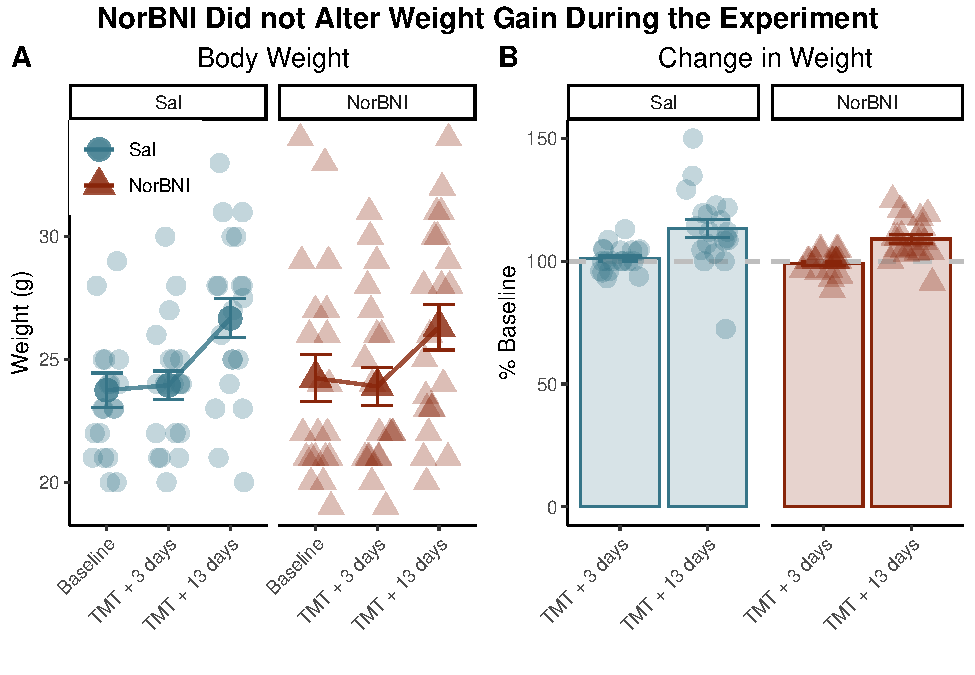
\includegraphics{_main_files/figure-latex/unnamed-chunk-4-1.pdf}

\hypertarget{graph-changes-in-body-weight}{%
\section{Graph changes in body weight}\label{graph-changes-in-body-weight}}

\begin{figure}
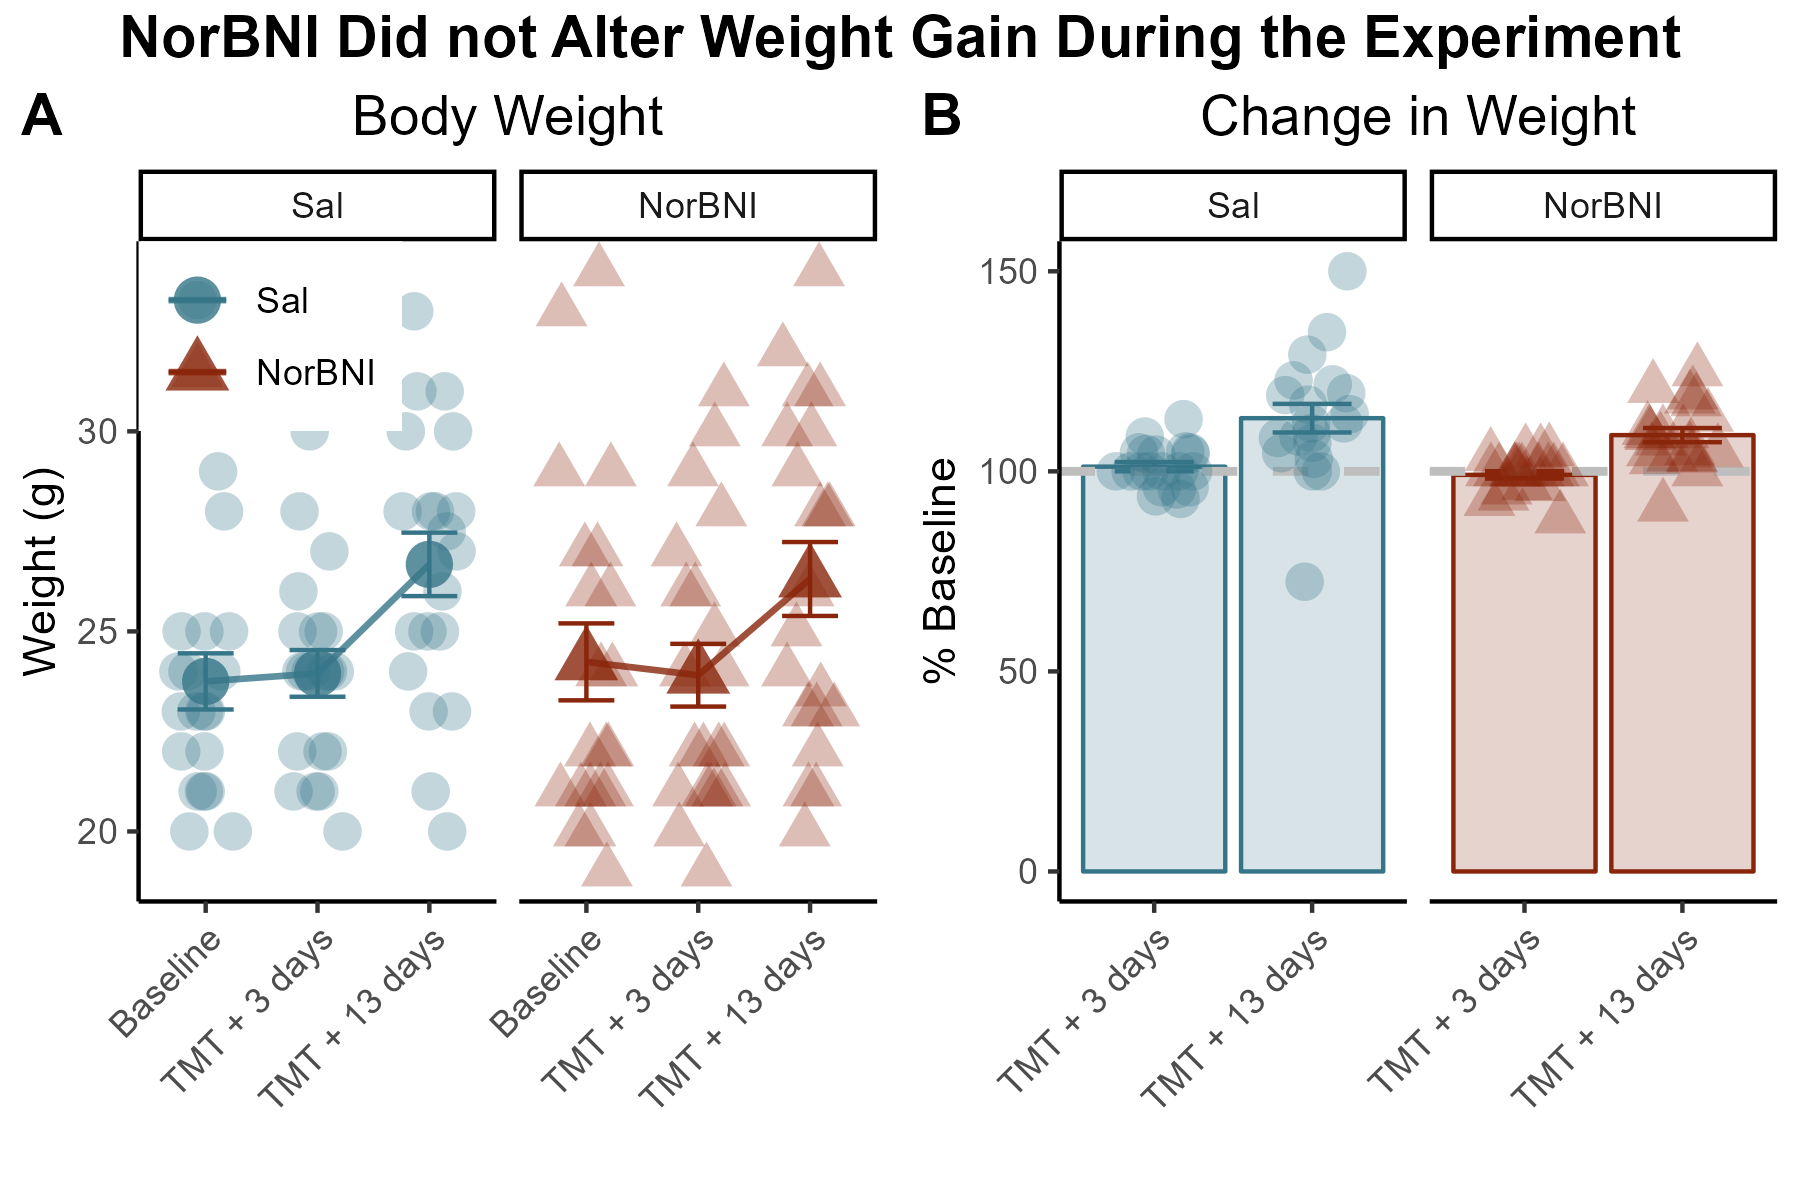
\includegraphics[width=25in]{Panels/Weights} \caption{(A) Raw weight measurements at each timepoint. (B) Weight data converted into a percentage of each mouse's individual baseline measruement.}\label{fig:unnamed-chunk-5}
\end{figure}

\hypertarget{analyze-changes-in-body-weight}{%
\section{Analyze changes in body weight}\label{analyze-changes-in-body-weight}}

\begin{Shaded}
\begin{Highlighting}[]
\CommentTok{\# Turn off scientific notation}
\FunctionTok{options}\NormalTok{(}\AttributeTok{scipen=}\DecValTok{999}\NormalTok{) }

\CommentTok{\# Run a one{-}way ANOVA on raw weights }
\NormalTok{c }\OtherTok{\textless{}{-}} \FunctionTok{aov}\NormalTok{(value}\SpecialCharTok{\textasciitilde{}}\NormalTok{variable}\SpecialCharTok{*}\NormalTok{Drug, }\AttributeTok{data=}\NormalTok{a)}

\CommentTok{\# Print out the result}
\FunctionTok{summary}\NormalTok{(c)}
\end{Highlighting}
\end{Shaded}

\begin{verbatim}
##                Df Sum Sq Mean Sq F value  Pr(>F)   
## variable        2  174.3   87.15   6.867 0.00151 **
## Drug            1    0.0    0.02   0.002 0.96805   
## variable:Drug   2    3.8    1.90   0.150 0.86079   
## Residuals     117 1484.7   12.69                   
## ---
## Signif. codes:  0 '***' 0.001 '**' 0.01 '*' 0.05 '.' 0.1 ' ' 1
\end{verbatim}

\begin{Shaded}
\begin{Highlighting}[]
\CommentTok{\# Run a one{-}way ANOVA on raw weights }
\NormalTok{c }\OtherTok{\textless{}{-}} \FunctionTok{aov}\NormalTok{(value}\SpecialCharTok{\textasciitilde{}}\NormalTok{variable}\SpecialCharTok{+}\NormalTok{Drug, }\AttributeTok{data=}\NormalTok{a)}

\CommentTok{\# Run post{-}hoc comparisons to investigate which timepoints are different}
\FunctionTok{TukeyHSD}\NormalTok{(c)}
\end{Highlighting}
\end{Shaded}

\begin{verbatim}
##   Tukey multiple comparisons of means
##     95% family-wise confidence level
## 
## Fit: aov(formula = value ~ variable + Drug, data = a)
## 
## $variable
##                       diff        lwr      upr     p adj
## TMT_3d-BL_wt   -0.07317073 -1.9271087 1.780767 0.9951743
## TMT_13D-BL_wt   2.48780488  0.6338669 4.341743 0.0052191
## TMT_13D-TMT_3d  2.56097561  0.7070376 4.414914 0.0038854
## 
## $Drug
##                  diff       lwr      upr    p adj
## NorBNI-Sal 0.02579365 -1.237474 1.289061 0.967818
\end{verbatim}

\hypertarget{interpret-changes-in-body-weight}{%
\section{Interpret changes in body weight}\label{interpret-changes-in-body-weight}}

\begin{itemize}
\item
  The main effect of day indicated that mice gained weight across the experiment (\emph{F}(2,119) = 6.97, \emph{p} = 0.001).
\item
  Post-hoc analyses indicated that mice gained weight between the baseline measurement and the 13-days post TMT measurement (\emph{p} = 0.005), but not between the baseline and the 3D timepoints (\emph{p} = 0.99).
\item
  NorBNI did not interact with change in weight gain across the timecourse (\emph{p} = 0.97).
\end{itemize}

\hypertarget{freezing-behaviour-during-tmt-presentation}{%
\chapter{Freezing Behaviour During TMT Presentation}\label{freezing-behaviour-during-tmt-presentation}}

\begin{figure}
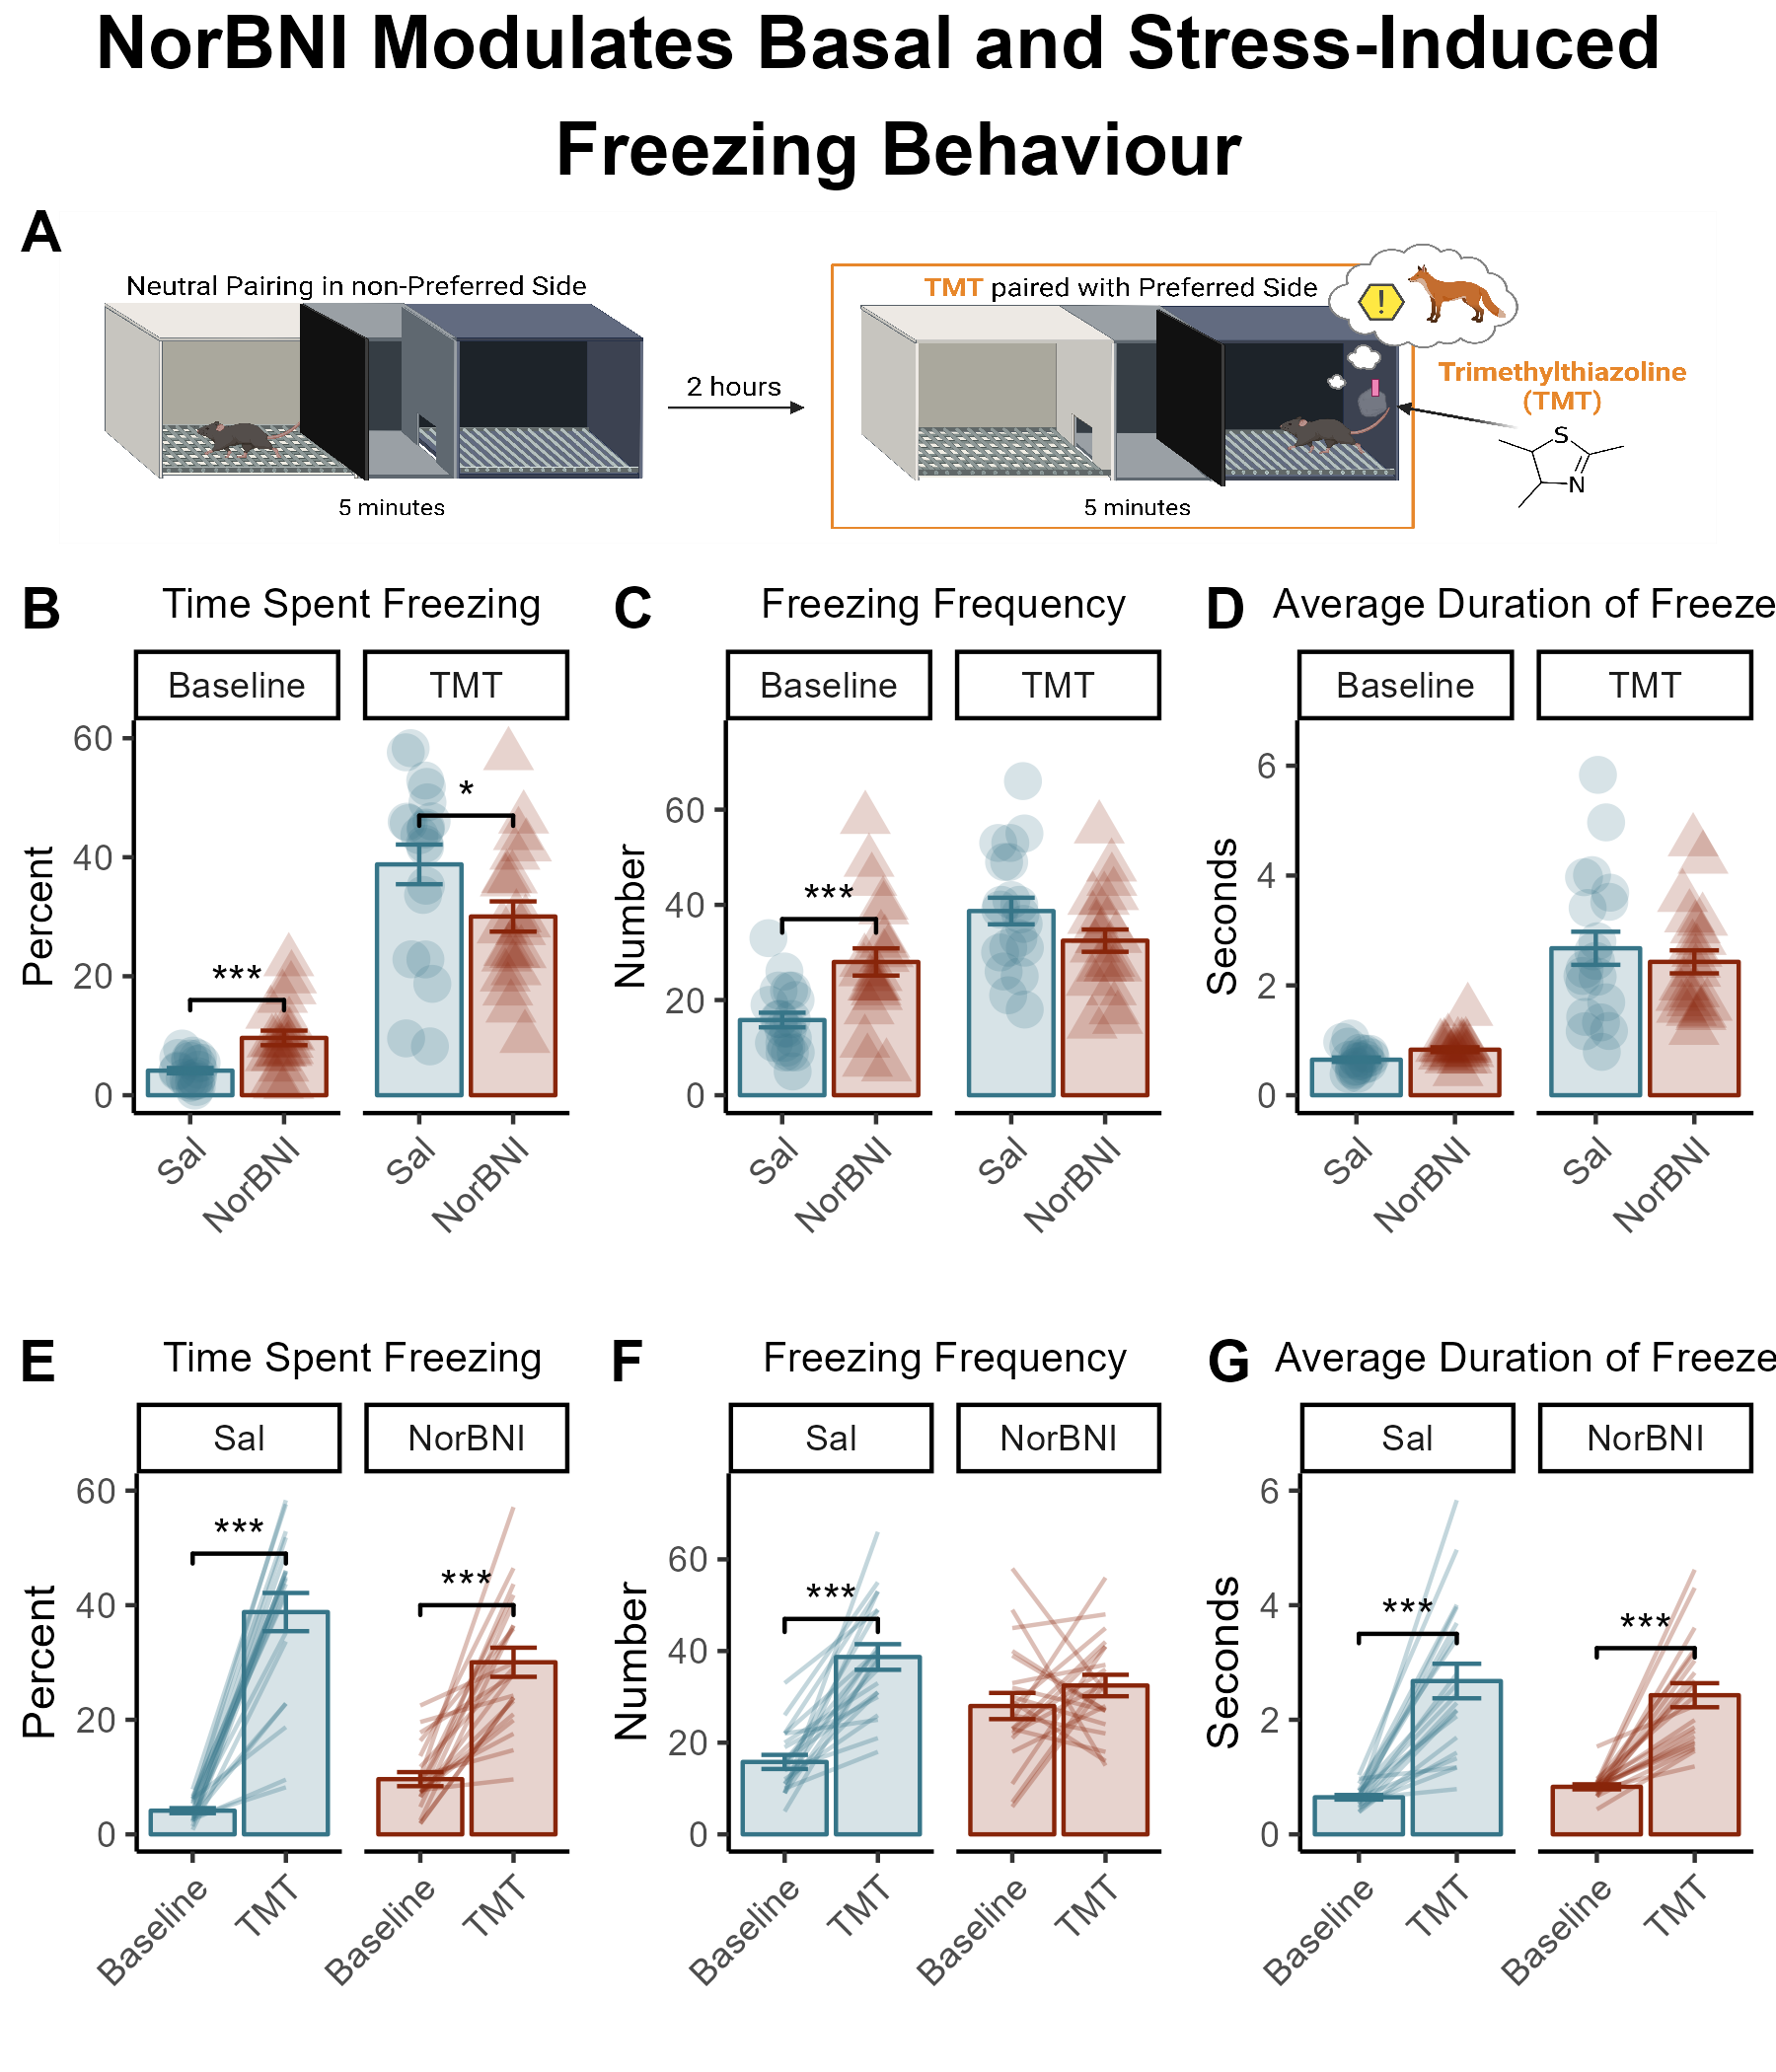
\includegraphics[width=25in]{Cartoons/Frz_Panel} \caption{Kappa-opioid receptor antagonism modulates basal and stress-induced freezing. (A) CPP was conducted such that each mouse was exposed to TMT for 5-minutes on their preferred side of the behavioural testing apparatus. (B) NorBNI administration 24hours before testing increases basal freezing and decreases freezing during TMT presentation. (C) The number of freezing episodes was increased at Neutral by NorBNI administration. (D) NorBNI did not produce any changes in the average duration of freezing episode under basal conditions or during TMT exposure. All mice exhibit an increase in the \% Freezing between the Neutral and TMT sessions (E), but only the saline group increased the number of freezing episodes between the two sessions (F). NorBNI administration did not affect the increase in average duration of freezing episode observed between the Neutral and TMT sessions (G). Data pressented as mean +/- SEM. * Indicates p < 0.05, *** indicates p < 0.001.}\label{fig:unnamed-chunk-10}
\end{figure}

\hypertarget{statistical-analyses}{%
\section{Statistical Analyses}\label{statistical-analyses}}

\hypertarget{two-way-anova-on-freezing-behaivour}{%
\subsection{Two-way ANOVA on Freezing behaivour}\label{two-way-anova-on-freezing-behaivour}}

\begin{Shaded}
\begin{Highlighting}[]
\NormalTok{a }\OtherTok{\textless{}{-}} \FunctionTok{aov}\NormalTok{(Frz\_Tm }\SpecialCharTok{\textasciitilde{}}\NormalTok{ Drug }\SpecialCharTok{*}\NormalTok{ Task, }\AttributeTok{data=}\NormalTok{train\_data)}
\FunctionTok{summary}\NormalTok{(a)}
\end{Highlighting}
\end{Shaded}

\begin{verbatim}
##             Df Sum Sq Mean Sq F value               Pr(>F)    
## Drug         1    340     340   0.555              0.45835    
## Task         1  95925   95925 156.610 < 0.0000000000000002 ***
## Drug:Task    1   6511    6511  10.631              0.00165 ** 
## Residuals   78  47776     613                                 
## ---
## Signif. codes:  0 '***' 0.001 '**' 0.01 '*' 0.05 '.' 0.1 ' ' 1
\end{verbatim}

We quantified freezing behaviour both during the neutral pairing and the TMT exposure to investigate whether Nor BNI administration affected basal or stress-induced levels of freezing.

We computed a 2x2 ANOVA with Drug (saline or Nor BNI) as the between-groups factor and timepoint (Neutral vs TMT) as the within-subjects variable. The omnibus test for this model indicated a significant main effect of timepoint (F(1,39) = 79.09, p \textless{} 0.001) and a timepoint * Drug interaction (F(1,39) = 11.41, p \textless{} 0.001). Follow- up comparisons of the significant interaction indicated that NorBNI-injected mice froze more than did controls during the Neutral exposure (p \textless{} 0.001) and that Nor-BNI-injected mice spent less time freezing than controls during the TMT exposure (p = 0.042). Nevertheless, both groups spent more time freeing during TMT presentation than they had at Neutral (both p \textless{} 0.001), suggesting that both groups exhibited an innate defensive response during the single 5-minute TMT session.

\begin{Shaded}
\begin{Highlighting}[]
\NormalTok{a }\OtherTok{\textless{}{-}} \FunctionTok{anova\_test}\NormalTok{(}\AttributeTok{data=}\NormalTok{train\_data, }\AttributeTok{dv=}\NormalTok{Frz\_Tm, }\AttributeTok{wid=}\NormalTok{ID, }\AttributeTok{within =}\NormalTok{ Task, }\AttributeTok{between =}\NormalTok{ Drug)}
\NormalTok{knitr}\SpecialCharTok{::}\FunctionTok{kable}\NormalTok{(}\FunctionTok{get\_anova\_table}\NormalTok{(a))}
\end{Highlighting}
\end{Shaded}

\begin{tabular}{l|r|r|r|r|l|r}
\hline
Effect & DFn & DFd & F & p & p<.05 & ges\\
\hline
Drug & 1 & 39 & 0.522 & 0.474 &  & 0.007\\
\hline
Task & 1 & 39 & 169.279 & 0.000 & * & 0.670\\
\hline
Drug:Task & 1 & 39 & 11.353 & 0.002 & * & 0.120\\
\hline
\end{tabular}

\begin{Shaded}
\begin{Highlighting}[]
\NormalTok{b }\OtherTok{\textless{}{-}}\NormalTok{ train\_data }\SpecialCharTok{\%\textgreater{}\%}
  \FunctionTok{group\_by}\NormalTok{(Drug)}\SpecialCharTok{\%\textgreater{}\%}
  \FunctionTok{pairwise\_t\_test}\NormalTok{(}
\NormalTok{  Frz\_Tm }\SpecialCharTok{\textasciitilde{}}\NormalTok{ Task, }\AttributeTok{paired =} \ConstantTok{TRUE}\NormalTok{,}
  \AttributeTok{p.adjust.method =} \StringTok{"bonferroni"}
\NormalTok{  )}

\NormalTok{knitr}\SpecialCharTok{::}\FunctionTok{kable}\NormalTok{(b)}
\end{Highlighting}
\end{Shaded}

\begin{tabular}{l|l|l|l|r|r|r|r|r|r|l}
\hline
Drug & .y. & group1 & group2 & n1 & n2 & statistic & df & p & p.adj & p.adj.signif\\
\hline
Saline & Frz\_Tm & Neutral & TMT & 20 & 20 & -10.722043 & 19 & 0.0000000 & 0.0000000 & ****\\
\hline
Nor-BNI & Frz\_Tm & Neutral & TMT & 21 & 21 & -7.409239 & 20 & 0.0000004 & 0.0000004 & ****\\
\hline
\end{tabular}

\begin{Shaded}
\begin{Highlighting}[]
\NormalTok{c }\OtherTok{\textless{}{-}}\NormalTok{ train\_data }\SpecialCharTok{\%\textgreater{}\%}
  \FunctionTok{group\_by}\NormalTok{(Task)}\SpecialCharTok{\%\textgreater{}\%}
  \FunctionTok{pairwise\_t\_test}\NormalTok{(}
\NormalTok{  Frz\_Tm }\SpecialCharTok{\textasciitilde{}}\NormalTok{ Drug, }\AttributeTok{paired =} \ConstantTok{FALSE}\NormalTok{,}
  \AttributeTok{p.adjust.method =} \StringTok{"bonferroni"}
\NormalTok{  )}

\NormalTok{knitr}\SpecialCharTok{::}\FunctionTok{kable}\NormalTok{(c)}
\end{Highlighting}
\end{Shaded}

\begin{tabular}{l|l|l|l|r|r|r|l|r|l}
\hline
Task & .y. & group1 & group2 & n1 & n2 & p & p.signif & p.adj & p.adj.signif\\
\hline
Neutral & Frz\_Tm & Saline & Nor-BNI & 20 & 21 & 0.000182 & *** & 0.000182 & ***\\
\hline
TMT & Frz\_Tm & Saline & Nor-BNI & 20 & 21 & 0.042000 & * & 0.042000 & *\\
\hline
\end{tabular}

We also computed ANOVA with the number of freezing episodes during each session entered as the dependent variable. This model also indicated a Drug * Timepoint interaction (F(1,39) = 13.17, p \textless{} 0.001). Saline-injected mice froze more often during the TMT session than the Neutral session (p \textless{} 0.001) whereas there was no difference in freezing frequency between the two sessions for NorBNI-injected mice (p = 0.28). Moreover, NorBNI-injected mice froze more often than did saline controls during the neutral exposure (p \textless{} 0.001), but there was no difference in freezing frequency between the groups during the TMT session (p = 0.09).

\begin{Shaded}
\begin{Highlighting}[]
\NormalTok{a }\OtherTok{\textless{}{-}} \FunctionTok{anova\_test}\NormalTok{(}\AttributeTok{data=}\NormalTok{train\_data, }\AttributeTok{dv=}\NormalTok{Frz\_Freq, }\AttributeTok{wid=}\NormalTok{ID, }\AttributeTok{within =}\NormalTok{ Task, }\AttributeTok{between =}\NormalTok{ Drug)}
\FunctionTok{get\_anova\_table}\NormalTok{(a)}
\end{Highlighting}
\end{Shaded}

\begin{verbatim}
## ANOVA Table (type III tests)
## 
##      Effect DFn DFd      F          p p<.05   ges
## 1      Drug   1  39  1.602 0.21300000       0.019
## 2      Task   1  39 29.078 0.00000361     * 0.286
## 3 Drug:Task   1  39 13.170 0.00081500     * 0.153
\end{verbatim}

\begin{Shaded}
\begin{Highlighting}[]
\NormalTok{b }\OtherTok{\textless{}{-}}\NormalTok{ train\_data }\SpecialCharTok{\%\textgreater{}\%}
  \FunctionTok{group\_by}\NormalTok{(Drug)}\SpecialCharTok{\%\textgreater{}\%}
  \FunctionTok{pairwise\_t\_test}\NormalTok{(}
\NormalTok{  Frz\_Freq }\SpecialCharTok{\textasciitilde{}}\NormalTok{ Task, }\AttributeTok{paired =} \ConstantTok{TRUE}\NormalTok{,}
  \AttributeTok{p.adjust.method =} \StringTok{"bonferroni"}
\NormalTok{  )}

\NormalTok{knitr}\SpecialCharTok{::}\FunctionTok{kable}\NormalTok{(b)}
\end{Highlighting}
\end{Shaded}

\begin{tabular}{l|l|l|l|r|r|r|r|r|r|l}
\hline
Drug & .y. & group1 & group2 & n1 & n2 & statistic & df & p & p.adj & p.adj.signif\\
\hline
Saline & Frz\_Freq & Neutral & TMT & 20 & 20 & -7.644742 & 19 & 0.0000003 & 0.0000003 & ****\\
\hline
Nor-BNI & Frz\_Freq & Neutral & TMT & 21 & 21 & -1.105378 & 20 & 0.2820000 & 0.2820000 & ns\\
\hline
\end{tabular}

\begin{Shaded}
\begin{Highlighting}[]
\NormalTok{c }\OtherTok{\textless{}{-}}\NormalTok{ train\_data }\SpecialCharTok{\%\textgreater{}\%}
  \FunctionTok{group\_by}\NormalTok{(Task)}\SpecialCharTok{\%\textgreater{}\%}
  \FunctionTok{pairwise\_t\_test}\NormalTok{(}
\NormalTok{  Frz\_Freq }\SpecialCharTok{\textasciitilde{}}\NormalTok{ Drug, }\AttributeTok{paired =} \ConstantTok{FALSE}\NormalTok{,}
  \AttributeTok{p.adjust.method =} \StringTok{"bonferroni"}
\NormalTok{  )}

\NormalTok{knitr}\SpecialCharTok{::}\FunctionTok{kable}\NormalTok{(c)}
\end{Highlighting}
\end{Shaded}

\begin{tabular}{l|l|l|l|r|r|r|l|r|l}
\hline
Task & .y. & group1 & group2 & n1 & n2 & p & p.signif & p.adj & p.adj.signif\\
\hline
Neutral & Frz\_Freq & Saline & Nor-BNI & 20 & 21 & 0.00065 & *** & 0.00065 & ***\\
\hline
TMT & Frz\_Freq & Saline & Nor-BNI & 20 & 21 & 0.09460 & ns & 0.09460 & ns\\
\hline
\end{tabular}

ANOVA on the average duration of freezing episode indicated a significant main effect of timepoint (F(1,39) = 103.45, p \textless{} 0.001) that did not interact with drug treatment (p = 0.24). The average duration of freezing episode was increased by TMT.

\begin{Shaded}
\begin{Highlighting}[]
\NormalTok{a }\OtherTok{\textless{}{-}} \FunctionTok{anova\_test}\NormalTok{(}\AttributeTok{data=}\NormalTok{train\_data, }\AttributeTok{dv=}\NormalTok{Av\_Dur, }\AttributeTok{wid=}\NormalTok{ID, }\AttributeTok{within =}\NormalTok{ Task, }\AttributeTok{between =}\NormalTok{ Drug)}
\FunctionTok{get\_anova\_table}\NormalTok{(a)}
\end{Highlighting}
\end{Shaded}

\begin{verbatim}
## ANOVA Table (type III tests)
## 
##      Effect DFn DFd       F                p p<.05      ges
## 1      Drug   1  39   0.029 0.86600000000000       0.000396
## 2      Task   1  39 103.456 0.00000000000158     * 0.553000
## 3 Drug:Task   1  39   1.452 0.23500000000000       0.017000
\end{verbatim}

\begin{Shaded}
\begin{Highlighting}[]
\NormalTok{b }\OtherTok{\textless{}{-}}\NormalTok{ train\_data }\SpecialCharTok{\%\textgreater{}\%}
  \FunctionTok{group\_by}\NormalTok{(Drug)}\SpecialCharTok{\%\textgreater{}\%}
  \FunctionTok{pairwise\_t\_test}\NormalTok{(}
\NormalTok{  Av\_Dur }\SpecialCharTok{\textasciitilde{}}\NormalTok{ Task, }\AttributeTok{paired =} \ConstantTok{TRUE}\NormalTok{,}
  \AttributeTok{p.adjust.method =} \StringTok{"bonferroni"}
\NormalTok{  )}

\NormalTok{knitr}\SpecialCharTok{::}\FunctionTok{kable}\NormalTok{(b)}
\end{Highlighting}
\end{Shaded}

\begin{tabular}{l|l|l|l|r|r|r|r|r|r|l}
\hline
Drug & .y. & group1 & group2 & n1 & n2 & statistic & df & p & p.adj & p.adj.signif\\
\hline
Saline & Av\_Dur & Neutral & TMT & 20 & 20 & -6.971897 & 19 & 0.0000012 & 0.0000012 & ****\\
\hline
Nor-BNI & Av\_Dur & Neutral & TMT & 21 & 21 & -7.589131 & 20 & 0.0000003 & 0.0000003 & ****\\
\hline
\end{tabular}

\begin{Shaded}
\begin{Highlighting}[]
\NormalTok{c }\OtherTok{\textless{}{-}}\NormalTok{ train\_data }\SpecialCharTok{\%\textgreater{}\%}
  \FunctionTok{group\_by}\NormalTok{(Task)}\SpecialCharTok{\%\textgreater{}\%}
  \FunctionTok{pairwise\_t\_test}\NormalTok{(}
\NormalTok{  Av\_Dur }\SpecialCharTok{\textasciitilde{}}\NormalTok{ Drug, }\AttributeTok{paired =} \ConstantTok{FALSE}\NormalTok{,}
  \AttributeTok{p.adjust.method =} \StringTok{"bonferroni"}
\NormalTok{  )}

\NormalTok{knitr}\SpecialCharTok{::}\FunctionTok{kable}\NormalTok{(c)}
\end{Highlighting}
\end{Shaded}

\begin{tabular}{l|l|l|l|r|r|r|l|r|l}
\hline
Task & .y. & group1 & group2 & n1 & n2 & p & p.signif & p.adj & p.adj.signif\\
\hline
Neutral & Av\_Dur & Saline & Nor-BNI & 20 & 21 & 0.00381 & ** & 0.00381 & **\\
\hline
TMT & Av\_Dur & Saline & Nor-BNI & 20 & 21 & 0.50100 & ns & 0.50100 & ns\\
\hline
\end{tabular}

Taken together, these findings indicate that NorBNI administration increases time spent freezing at Neutral by increasing the frequency of bouts of freezing. TMT exposure increases both the frequency and average duration of bouts of freezing among naive mice, and the magnitude of the change in freezing behaviour is reduced among NorBNI treated mice.

\hypertarget{regressions}{%
\subsection{Regressions}\label{regressions}}

\begin{verbatim}
## 
## Call:
## lm(formula = Perc ~ Frz_Freq * Drug, data = BL_data)
## 
## Residuals:
##     Min      1Q  Median      3Q     Max 
## -2.8267 -0.7702 -0.1686  0.3901  8.3884 
## 
## Coefficients:
##                      Estimate Std. Error t value Pr(>|t|)    
## (Intercept)           0.35976    1.03281   0.348 0.729567    
## Frz_Freq              0.23889    0.06017   3.970 0.000318 ***
## DrugNor-BNI          -1.78723    1.40227  -1.275 0.210422    
## Frz_Freq:DrugNor-BNI  0.15621    0.06761   2.311 0.026535 *  
## ---
## Signif. codes:  0 '***' 0.001 '**' 0.01 '*' 0.05 '.' 0.1 ' ' 1
## 
## Residual standard error: 1.804 on 37 degrees of freedom
## Multiple R-squared:  0.8815, Adjusted R-squared:  0.8719 
## F-statistic: 91.78 on 3 and 37 DF,  p-value: < 0.00000000000000022
\end{verbatim}

\begin{verbatim}
## 
## Call:
## lm(formula = Perc ~ Frz_Freq * Drug, data = b)
## 
## Residuals:
##     Min      1Q  Median      3Q     Max 
## -2.8267 -0.7702 -0.1686  0.3901  8.3884 
## 
## Coefficients:
##                     Estimate Std. Error t value            Pr(>|t|)    
## (Intercept)         -1.42747    0.94851  -1.505              0.1408    
## Frz_Freq             0.39510    0.03082  12.820 0.00000000000000351 ***
## DrugSaline           1.78723    1.40227   1.275              0.2104    
## Frz_Freq:DrugSaline -0.15621    0.06761  -2.311              0.0265 *  
## ---
## Signif. codes:  0 '***' 0.001 '**' 0.01 '*' 0.05 '.' 0.1 ' ' 1
## 
## Residual standard error: 1.804 on 37 degrees of freedom
## Multiple R-squared:  0.8815, Adjusted R-squared:  0.8719 
## F-statistic: 91.78 on 3 and 37 DF,  p-value: < 0.00000000000000022
\end{verbatim}

A regression model with Percent freezing during the Neutral session entered as the dependent variable and freezing frequency entered as the independent variable accounted for 87\% of the variability in freezing (F(3,37) = 91.78, Adjusted R\^{}2 = 0.87, p \textless{} 0.001). Simple effects for this model indicated a significant main effect of Freezing Frequency (t = 3.97, p \textless{} 0.001) and a significant Frequency * Drug interaction (t = 2.33, p = 0.026). Evaluation of the simple slopes for each drug condition indicated that for saline-treated mice, a 10-unit increase in freezing frequency was associated with a 2.3\% increase in total time freezing. Among NorBNI-treated mice, a 10-unit increase in freezing was associated with a 3.9\% increase in total time freezing.

\begin{verbatim}
## 
## Call:
## lm(formula = Perc ~ Frz_Freq * Drug, data = TMTs)
## 
## Residuals:
##      Min       1Q   Median       3Q      Max 
## -26.5697  -7.2100   0.5262   9.3678  23.8668 
## 
## Coefficients:
##                      Estimate Std. Error t value Pr(>|t|)   
## (Intercept)           26.5527     9.5304   2.786  0.00837 **
## Frz_Freq               0.3165     0.2349   1.347  0.18607   
## DrugNor-BNI          -12.8500    13.1699  -0.976  0.33554   
## Frz_Freq:DrugNor-BNI   0.1866     0.3551   0.525  0.60249   
## ---
## Signif. codes:  0 '***' 0.001 '**' 0.01 '*' 0.05 '.' 0.1 ' ' 1
## 
## Residual standard error: 12.79 on 37 degrees of freedom
## Multiple R-squared:  0.2159, Adjusted R-squared:  0.1523 
## F-statistic: 3.395 on 3 and 37 DF,  p-value: 0.02779
\end{verbatim}

\begin{Shaded}
\begin{Highlighting}[]
\CommentTok{\# Model 2: X=Av\_Dur, y=Perc}
\NormalTok{a }\OtherTok{\textless{}{-}} \FunctionTok{lm}\NormalTok{(Perc}\SpecialCharTok{\textasciitilde{}}\NormalTok{Av\_Dur }\SpecialCharTok{*}\NormalTok{ Drug, }\AttributeTok{data=}\NormalTok{BL\_data)}
\FunctionTok{summary}\NormalTok{(a)}
\end{Highlighting}
\end{Shaded}

\begin{verbatim}
## 
## Call:
## lm(formula = Perc ~ Av_Dur * Drug, data = BL_data)
## 
## Residuals:
##     Min      1Q  Median      3Q     Max 
## -7.8633 -1.6178 -0.8294  1.2113 10.2455 
## 
## Coefficients:
##                    Estimate Std. Error t value Pr(>|t|)  
## (Intercept)         -0.1638     2.8444  -0.058   0.9544  
## Av_Dur               6.6422     4.2461   1.564   0.1263  
## DrugNor-BNI         -5.6693     4.2286  -1.341   0.1882  
## Av_Dur:DrugNor-BNI  12.0048     5.6131   2.139   0.0391 *
## ---
## Signif. codes:  0 '***' 0.001 '**' 0.01 '*' 0.05 '.' 0.1 ' ' 1
## 
## Residual standard error: 3.292 on 37 degrees of freedom
## Multiple R-squared:  0.6058, Adjusted R-squared:  0.5738 
## F-statistic: 18.95 on 3 and 37 DF,  p-value: 0.00000013
\end{verbatim}

\begin{Shaded}
\begin{Highlighting}[]
\CommentTok{\# Re{-}order the "drug" variable to get the intercept for the NorBNI group.}
\NormalTok{b }\OtherTok{\textless{}{-}}\NormalTok{ BL\_data}
\NormalTok{b}\SpecialCharTok{$}\NormalTok{Drug }\OtherTok{\textless{}{-}} \FunctionTok{as.character}\NormalTok{(b}\SpecialCharTok{$}\NormalTok{Drug)}
\NormalTok{b}\SpecialCharTok{$}\NormalTok{Drug }\OtherTok{\textless{}{-}} \FunctionTok{factor}\NormalTok{(b}\SpecialCharTok{$}\NormalTok{Drug,}\AttributeTok{levels =} \FunctionTok{c}\NormalTok{(}\StringTok{"Nor{-}BNI"}\NormalTok{,}\StringTok{"Saline"}\NormalTok{))}

\CommentTok{\# A regression model on Neutral Freezing}
\NormalTok{a }\OtherTok{\textless{}{-}} \FunctionTok{lm}\NormalTok{(Perc}\SpecialCharTok{\textasciitilde{}}\NormalTok{Av\_Dur }\SpecialCharTok{*}\NormalTok{ Drug, }\AttributeTok{data=}\NormalTok{b)}
\FunctionTok{summary}\NormalTok{(a)}
\end{Highlighting}
\end{Shaded}

\begin{verbatim}
## 
## Call:
## lm(formula = Perc ~ Av_Dur * Drug, data = b)
## 
## Residuals:
##     Min      1Q  Median      3Q     Max 
## -7.8633 -1.6178 -0.8294  1.2113 10.2455 
## 
## Coefficients:
##                   Estimate Std. Error t value Pr(>|t|)    
## (Intercept)         -5.833      3.129  -1.864   0.0702 .  
## Av_Dur              18.647      3.671   5.079 0.000011 ***
## DrugSaline           5.669      4.229   1.341   0.1882    
## Av_Dur:DrugSaline  -12.005      5.613  -2.139   0.0391 *  
## ---
## Signif. codes:  0 '***' 0.001 '**' 0.01 '*' 0.05 '.' 0.1 ' ' 1
## 
## Residual standard error: 3.292 on 37 degrees of freedom
## Multiple R-squared:  0.6058, Adjusted R-squared:  0.5738 
## F-statistic: 18.95 on 3 and 37 DF,  p-value: 0.00000013
\end{verbatim}

\hypertarget{conditioned-place-aversion-to-tmt}{%
\chapter{Conditioned Place Aversion to TMT}\label{conditioned-place-aversion-to-tmt}}

\begin{figure}
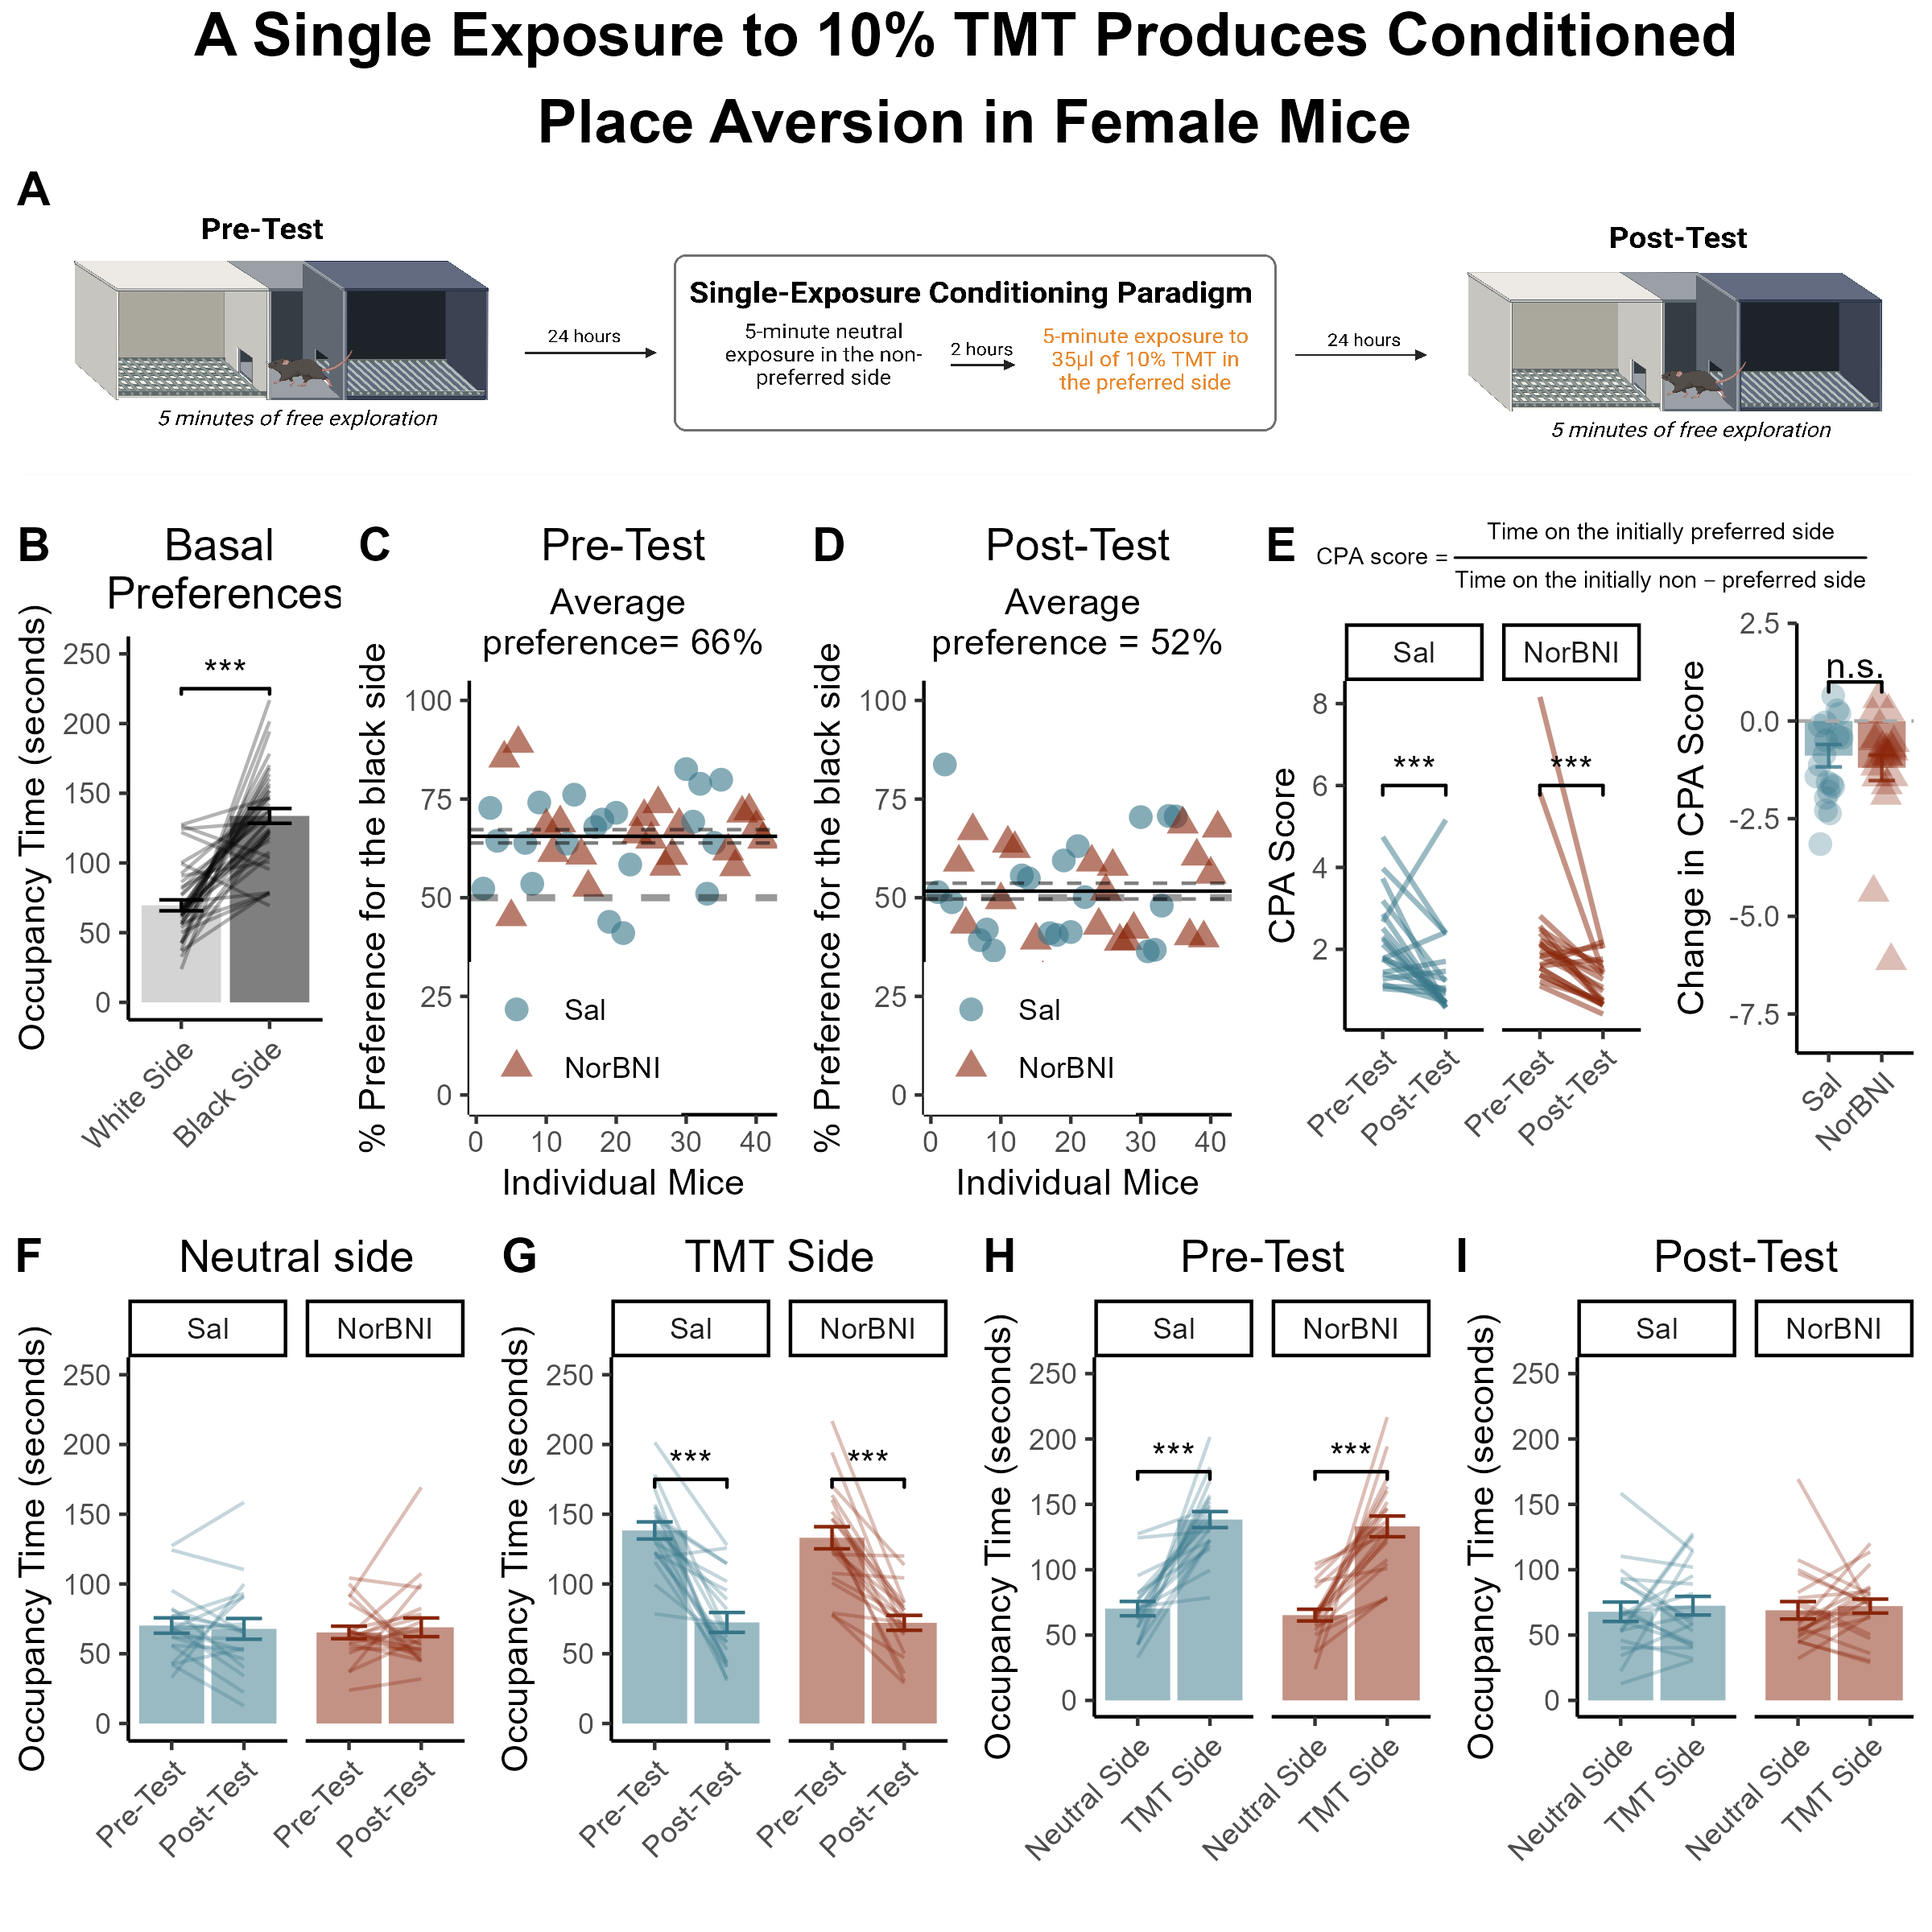
\includegraphics[width=33.33in]{Panels/CPA_panel} \caption{Timeline of experimental proceedings for Conditioned Place Aversion (A). The Conditioning apparatus used in these epxeriments was biased, such that mice exhibit an overall preference for the black compartment over the white compartment under basal conditions (B,C). The preference for the black compartment was reduced after the training session with TMT (D). Mice exhibited conditioned place aversion between the pre-test and the post-test (E) Which was not altered by NorBNI (F). Between the pre-test and the post-test, mice reduced time spent on the TMT-paried side (G) but did not exhibit a change in time spent on the netutral side (H). The strong side preferences that were observed during the Pre-test (I) were ablated by the single paring with TMT (J). Data presented as mean value +/- SEM, *** indicates p < 0.001.}\label{fig:unnamed-chunk-29}
\end{figure}

\hypertarget{statistical-analyses-1}{%
\section{Statistical Analyses}\label{statistical-analyses-1}}

We conducted an initial preference test to evaluate each mouse's preferred side of the CPP apparatus. Time spent in each of the 3 compartments was scored manually. We found that overall, mice preferred the black side of the apparatus over the white side (paired t(40) = 8.53, p \textless{} 0.001).

\begin{verbatim}
## 
##  Paired t-test
## 
## data:  BL_black_time and BL_white_time
## t = 8.5259, df = 40, p-value = 0.0000000001553
## alternative hypothesis: true mean difference is not equal to 0
## 95 percent confidence interval:
##  48.93262 79.33958
## sample estimates:
## mean difference 
##         64.1361
\end{verbatim}

Indeed, 38 / 41 mice tested in these experiments spent more time on the black side of the apparatus than the white side during the baseline test. Each mouse was exposed to TMT on the side that it exhibited a preference for during the baseline test (i.e.~38 of 41 mice were exposed to TMT on the black side of the apparatus; see figure XXX).

but did not exhibit a change in time spent in the neutral (non-preferred) compartment (p = 0.88).

\begin{verbatim}
## 
##  Paired t-test
## 
## data:  Baseline_tm_NON_PREF and Post_tm_NON_PREF
## t = -0.15062, df = 40, p-value = 0.881
## alternative hypothesis: true mean difference is not equal to 0
## 95 percent confidence interval:
##  -10.352845   8.916748
## sample estimates:
## mean difference 
##      -0.7180488
\end{verbatim}

To investigate chagnes in occupancy time between the Pre-test and the Post-test, computed a 3-way mixed model ANOVA with Task (pre-test or post-test) and Side (preferred or non-preferred) entered as the within-subjects variables, and Drug condition (Sailne or NorBNI) entered as a between-groups factor. The model indicated a significant Task * Side interaction (F(1,39) = 76.52, p \textless{} 0.001).

\begin{tabular}{l|r|r|r|r|l|r}
\hline
Effect & DFn & DFd & F & p & p<.05 & ges\\
\hline
Drug & 1 & 39 & 0.214 & 0.646 &  & 0.0020000\\
\hline
Task & 1 & 39 & 59.793 & 0.000 & * & 0.2350000\\
\hline
Side & 1 & 39 & 48.177 & 0.000 & * & 0.2870000\\
\hline
Drug:Task & 1 & 39 & 0.461 & 0.501 &  & 0.0020000\\
\hline
Drug:Side & 1 & 39 & 0.007 & 0.936 &  & 0.0000544\\
\hline
Task:Side & 1 & 39 & 76.520 & 0.000 & * & 0.2420000\\
\hline
Drug:Task:Side & 1 & 39 & 0.006 & 0.939 &  & 0.0000250\\
\hline
\end{tabular}

Follow-up analyses of the significant interaction indicated that mice exhibited robust preferences during the baseline session (t(41) = 10.27, p \textless{} 0.001) and that the preferences were not present during the post-test session (p = 0.51). Moreover, Mice decreased the amount of time spent on the initially prefrred side of the apparatus between the pre-test and the post-test (t(41) = 10.57, p \textless{} 0.001) but there was no change in occupancy time on the non-preferred side between the two sessions (p = 0.88). The 3-way interaction between Drug, Task and Side was non-significant (p = 0.94), indicating that kappa opioid antagonism did not alter the induction or the expression of conditioned place aversion to TMT in female mice.

\begin{tabular}{l|l|l|l|r|r|r|r|r|r|l}
\hline
Task & .y. & group1 & group2 & n1 & n2 & statistic & df & p & p.adj & p.adj.signif\\
\hline
Post & value & Preferred & Non-Preferred & 41 & 41 & 0.6629701 & 40 & 0.511 & 0.511 & ns\\
\hline
Pre & value & Preferred & Non-Preferred & 41 & 41 & 10.2746859 & 40 & 0.000 & 0.000 & ****\\
\hline
\end{tabular}

\begin{tabular}{l|l|l|l|r|r|r|r|r|r|l}
\hline
Side & .y. & group1 & group2 & n1 & n2 & statistic & df & p & p.adj & p.adj.signif\\
\hline
Preferred & value & Post & Pre & 41 & 41 & -10.5721883 & 40 & 0.000 & 0.000 & ****\\
\hline
Non-Preferred & value & Post & Pre & 41 & 41 & 0.1506239 & 40 & 0.881 & 0.881 & ns\\
\hline
\end{tabular}

We also computed ``CPA Scores'' which represent the \emph{ratio} of time on the preferred side to the non-preferred side:

\[CPA \; score = \frac{time \;on \;the \;preferred \;side}{time \;on \;the \;non-preferred \;side}\]

We found a significant effect of timepoint on CPA scores such that the ratio decreased between the pre-test and the post-test (F(1,39) = 22.67, p \textless{} 0.001)

\begin{tabular}{l|r|r|r|r|l|r}
\hline
Effect & DFn & DFd & F & p & p<.05 & ges\\
\hline
Drug & 1 & 39 & 0.007 & 0.9330000 &  & 0.000115\\
\hline
variable & 1 & 39 & 22.666 & 0.0000266 & * & 0.178000\\
\hline
Drug:variable & 1 & 39 & 0.498 & 0.4850000 &  & 0.005000\\
\hline
\end{tabular}

The magnitude of the change in CPA score was not different for NorBNI-treated mice (p = 0.48).

\begin{verbatim}
## 
##  Welch Two Sample t-test
## 
## data:  CPA_change_score by Drug
## t = 0.70831, df = 38.579, p-value = 0.483
## alternative hypothesis: true difference in means between group Sal and group NorBNI is not equal to 0
## 95 percent confidence interval:
##  -0.5736782  1.1916416
## sample estimates:
##    mean in group Sal mean in group NorBNI 
##           -0.8879249           -1.1969066
\end{verbatim}

\hypertarget{elevated-plus-maze}{%
\chapter{Elevated Plus Maze}\label{elevated-plus-maze}}

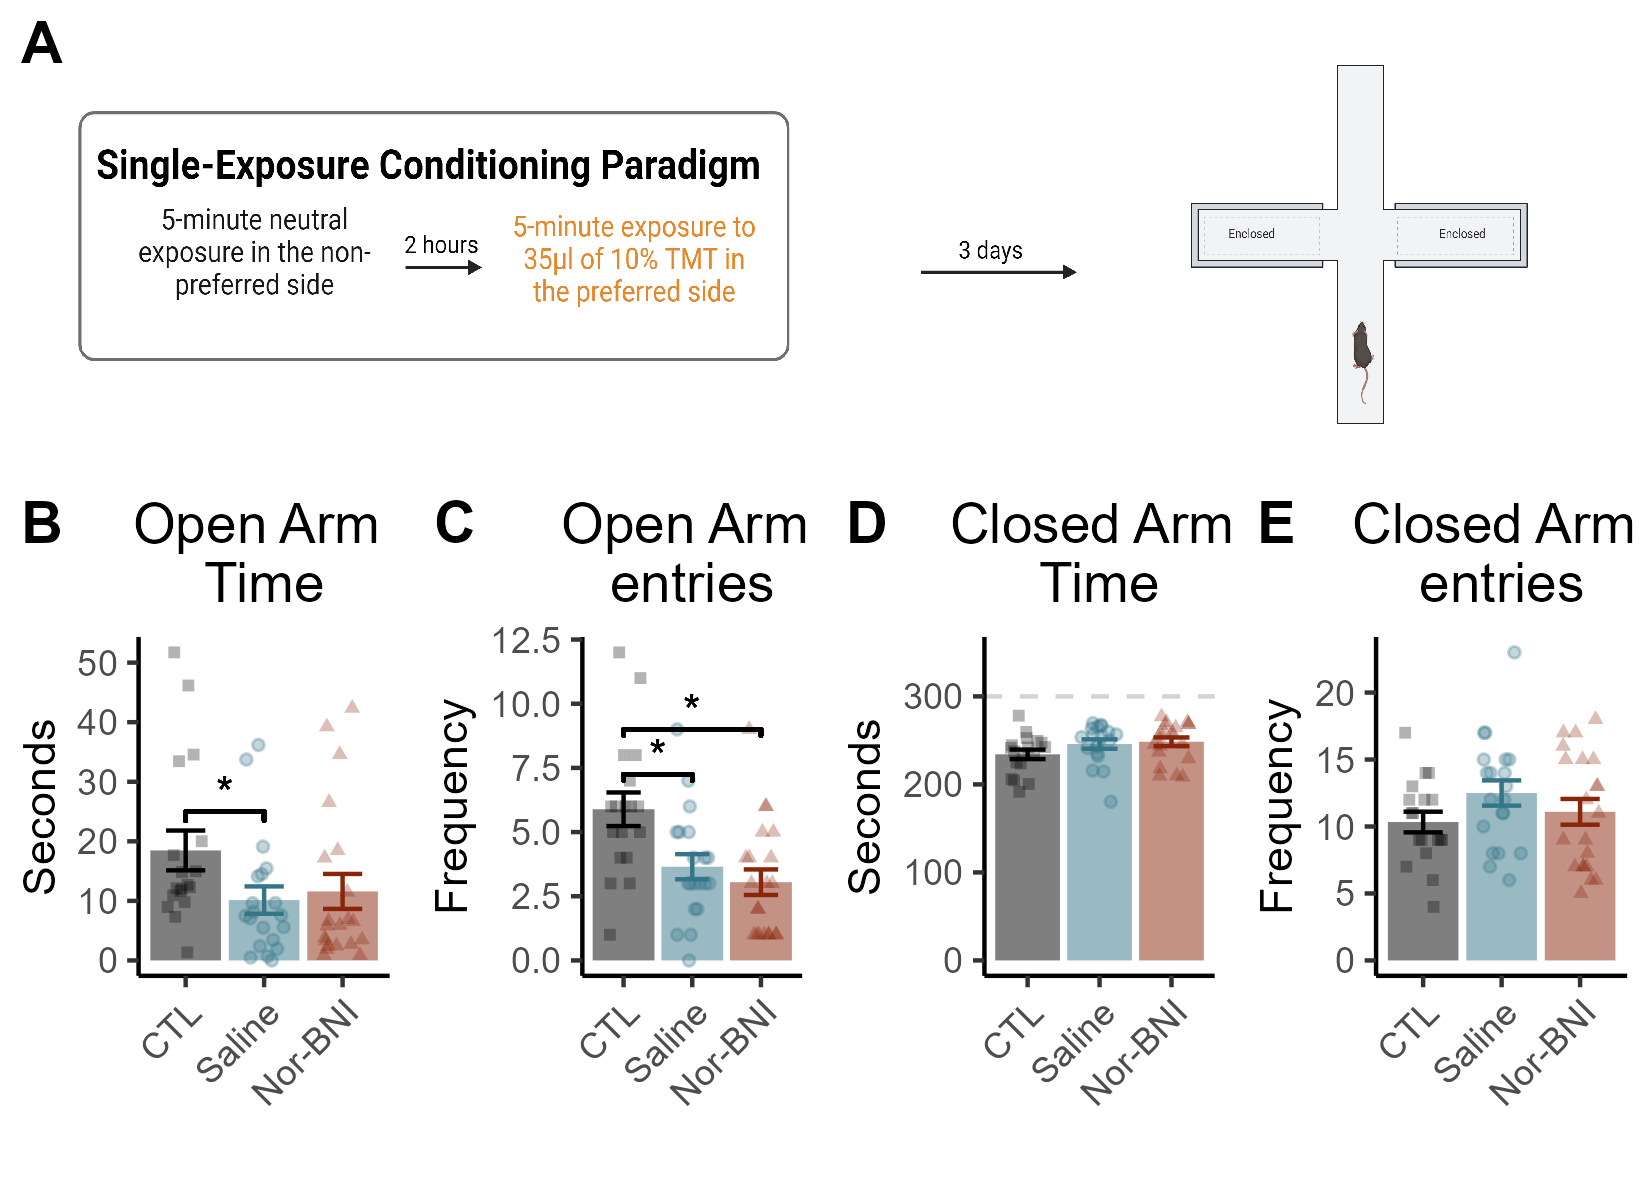
\includegraphics[width=22.92in]{Panels/EPM_panel}

\hypertarget{statistical-analyses-2}{%
\section{Statistical Analyses}\label{statistical-analyses-2}}

One-way ANOVA on time spent in the open arm indicated a significant effect of group (F(1,57) = 4.78, p = 0.03).

\begin{verbatim}
## 
##  One-way analysis of means
## 
## data:  Open_Tm and TMT
## F = 4.7778, num df = 1, denom df = 57, p-value = 0.03295
\end{verbatim}

\begin{tabular}{l|l|l|r|r|r|l|r|l}
\hline
.y. & group1 & group2 & n1 & n2 & p & p.signif & p.adj & p.adj.signif\\
\hline
Open\_Tm & CTL & Saline & 18 & 20 & 0.0428 & * & 0.128 & ns\\
\hline
Open\_Tm & CTL & Nor-BNI & 18 & 21 & 0.0889 & ns & 0.267 & ns\\
\hline
Open\_Tm & Saline & Nor-BNI & 20 & 21 & 0.7080 & ns & 1.000 & ns\\
\hline
\end{tabular}

One-way ANOVA on time the number of entries into the open arm indicated a significant effect of group (F(1,57) = 14.78, p \textless{} 0.001)

\begin{verbatim}
## 
##  One-way analysis of means
## 
## data:  Open_Freq and TMT
## F = 14.782, num df = 1, denom df = 57, p-value = 0.0003064
\end{verbatim}

\begin{verbatim}
## 
##  One-way analysis of means
## 
## data:  Open_Tm and TMT
## F = 4.7778, num df = 1, denom df = 57, p-value = 0.03295
\end{verbatim}

\begin{tabular}{l|l|l|r|r|r|l|r|l}
\hline
.y. & group1 & group2 & n1 & n2 & p & p.signif & p.adj & p.adj.signif\\
\hline
Open\_Freq & CTL & Saline & 18 & 20 & 0.004870 & ** & 0.01460 & *\\
\hline
Open\_Freq & CTL & Nor-BNI & 18 & 21 & 0.000403 & *** & 0.00121 & **\\
\hline
Open\_Freq & Saline & Nor-BNI & 20 & 21 & 0.415000 & ns & 1.00000 & ns\\
\hline
\end{tabular}

Follow-up pairwise comparisons indicated that CTL mice made more entries into the open arms than TMT+Saline (p = 0.005) or TMT+NorBNI (p \textless{} 0.001) mice, and that there was no effect of NorBNI treatment among TMT-exposed mice (p = 0.41)

There were no differences in time spent in the closed arms or number of enteries into the closed arms.

\begin{verbatim}
## 
##  One-way analysis of means
## 
## data:  Closed_Tm and TMT
## F = 1.2163, num df = 1, denom df = 57, p-value = 0.2747
\end{verbatim}

\begin{verbatim}
## 
##  One-way analysis of means
## 
## data:  Open_Tm and TMT
## F = 4.7778, num df = 1, denom df = 57, p-value = 0.03295
\end{verbatim}

\begin{tabular}{l|l|l|r|r|r|l|r|l}
\hline
.y. & group1 & group2 & n1 & n2 & p & p.signif & p.adj & p.adj.signif\\
\hline
Closed\_Tm & CTL & Saline & 18 & 20 & 0.677 & ns & 1.000 & ns\\
\hline
Closed\_Tm & CTL & Nor-BNI & 18 & 21 & 0.141 & ns & 0.422 & ns\\
\hline
Closed\_Tm & Saline & Nor-BNI & 20 & 21 & 0.276 & ns & 0.827 & ns\\
\hline
\end{tabular}

\begin{verbatim}
## 
##  One-way analysis of means
## 
## data:  Closed_Freq and TMT
## F = 1.691, num df = 1, denom df = 57, p-value = 0.1987
\end{verbatim}

\begin{verbatim}
## 
##  One-way analysis of means
## 
## data:  Open_Tm and TMT
## F = 4.7778, num df = 1, denom df = 57, p-value = 0.03295
\end{verbatim}

\begin{tabular}{l|l|l|r|r|r|l|r|l}
\hline
.y. & group1 & group2 & n1 & n2 & p & p.signif & p.adj & p.adj.signif\\
\hline
Closed\_Freq & CTL & Saline & 18 & 20 & 0.0949 & ns & 0.285 & ns\\
\hline
Closed\_Freq & CTL & Nor-BNI & 18 & 21 & 0.5480 & ns & 1.000 & ns\\
\hline
Closed\_Freq & Saline & Nor-BNI & 20 & 21 & 0.2570 & ns & 0.771 & ns\\
\hline
\end{tabular}

\begin{verbatim}
## 
##  One-way analysis of means
## 
## data:  exp_index and TMT
## F = 11.698, num df = 1, denom df = 57, p-value = 0.001163
\end{verbatim}

\begin{verbatim}
## 
##  One-way analysis of means
## 
## data:  Open_Tm and TMT
## F = 4.7778, num df = 1, denom df = 57, p-value = 0.03295
\end{verbatim}

\begin{tabular}{l|l|l|r|r|r|l|r|l}
\hline
.y. & group1 & group2 & n1 & n2 & p & p.signif & p.adj & p.adj.signif\\
\hline
exp\_index & CTL & Saline & 18 & 20 & 0.00474 & ** & 0.0142 & *\\
\hline
exp\_index & CTL & Nor-BNI & 18 & 21 & 0.00411 & ** & 0.0123 & *\\
\hline
exp\_index & Saline & Nor-BNI & 20 & 21 & 0.98600 & ns & 1.0000 & ns\\
\hline
\end{tabular}

\hypertarget{basal-freezing-long-after-tmt}{%
\chapter{Basal Freezing Long After TMT}\label{basal-freezing-long-after-tmt}}

\begin{figure}
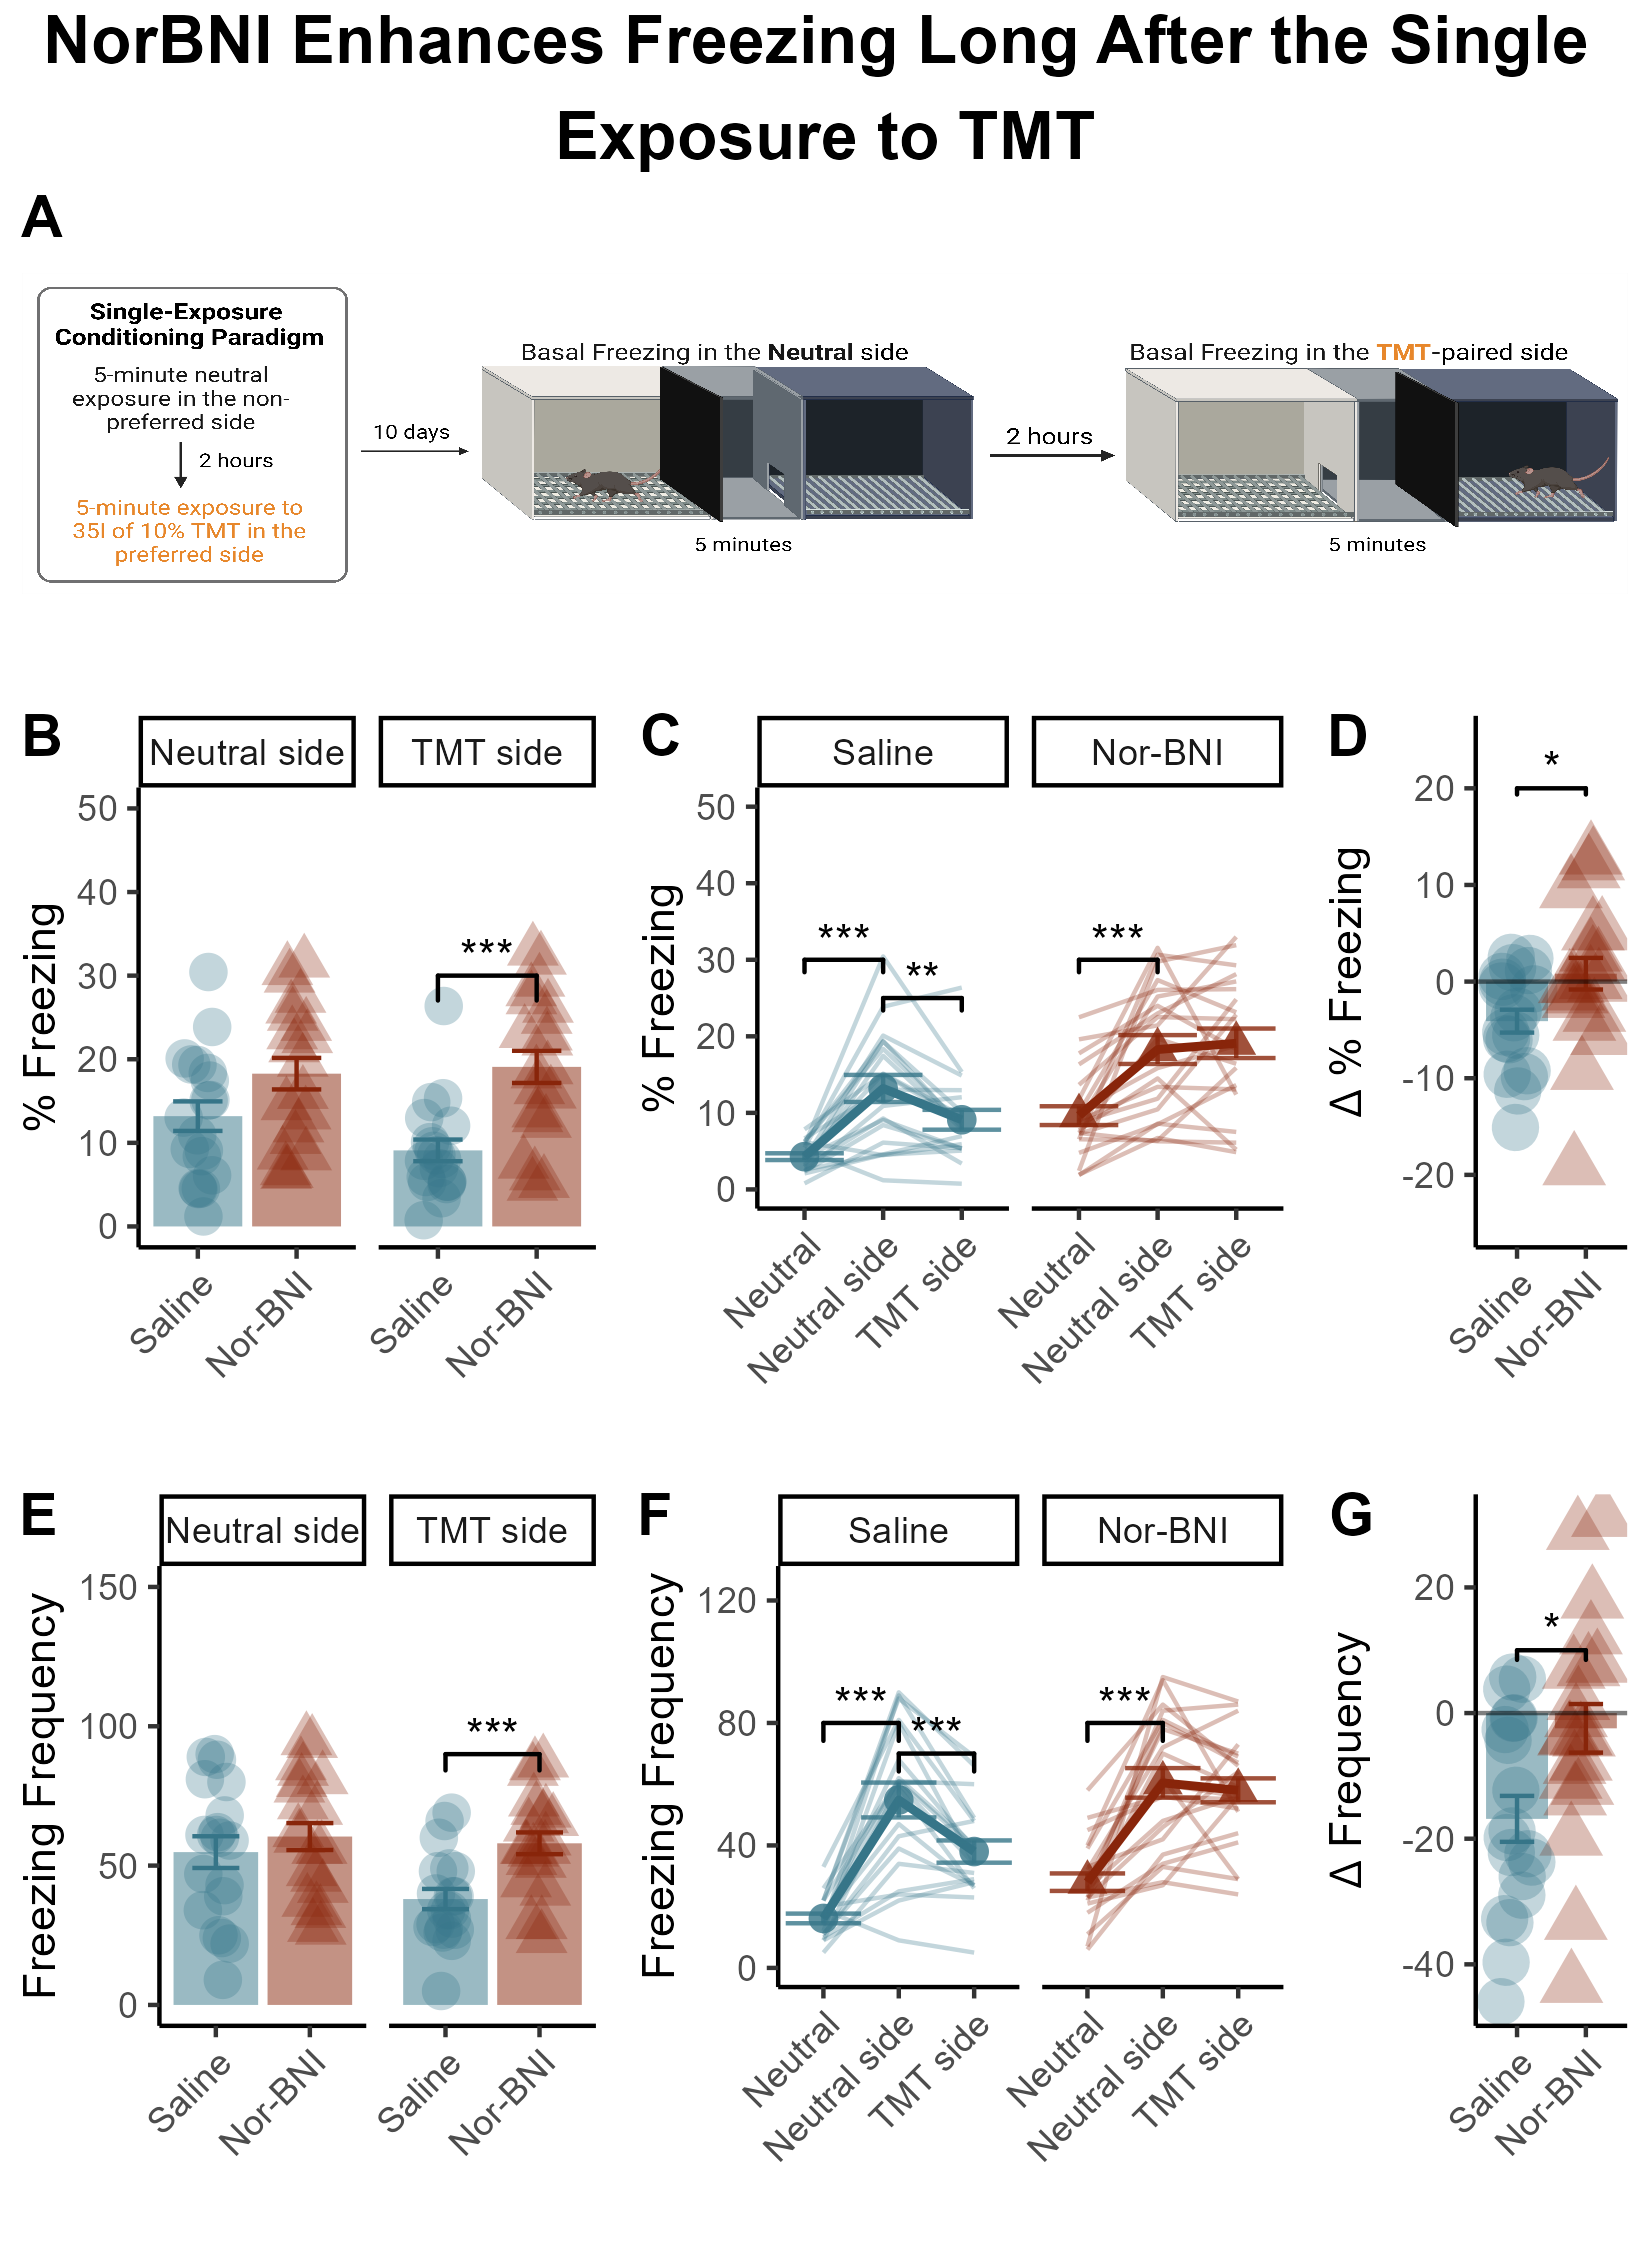
\includegraphics[width=22.92in]{Panels/Long_Panel} \caption{Timeline of experimental proceedings: 10 days after the single 5-minute exposure to 10\% TMT, mice were placed in each side of the conditioning apparatus for 5 minutes and basal levels of freezing were measured (A). Nor-BNI injected mice froze more than saline mice on the TMT-paired side, but not on the neutral side (B). Both drug conditions exhibited a robust increase in freezing relative to their baseline data from 10 days earlier (C). Saline mice decreased freezing between the two sessions whereas NorBNI-treated mice did not (C). The change in freezing behaviour between the two sessions was significantly reduced by NorBNI administration (D). The frequency of freezing was significantly higher for NorBNI injected mice on the TMT-paried side, but not the neutral side (E). Saline but not NorBNI injected mice reduced the frequency of freezing between the two sessions (F). The magnitude of the change between the two sessions was significantly reduced by NorBNI (G). Data presented as mean +/- SEM, * p < 0.05, ** p < 0.01, *** p < 0.001. }\label{fig:unnamed-chunk-58}
\end{figure}

\hypertarget{statistical-analyses-3}{%
\section{Statistical Analyses}\label{statistical-analyses-3}}

\hypertarget{time-spent-freezing}{%
\subsection{Time Spent Freezing}\label{time-spent-freezing}}

We computed a 2x2 ANOVA with side (Neutral or TMT-paired) as the within subjects factor and Drug condition (Saline or NorBNI) as the between groups factor. This model indicated a significant side * Drug interaction (F(1,38) = 5.69, p = 0.02)

\begin{tabular}{l|r|r|r|r|l|r}
\hline
Effect & DFn & DFd & F & p & p<.05 & ges\\
\hline
Drug & 1 & 38 & 11.071 & 0.002 & * & 0.195\\
\hline
variable & 1 & 38 & 2.542 & 0.119 &  & 0.011\\
\hline
Drug:variable & 1 & 38 & 5.693 & 0.022 & * & 0.025\\
\hline
\end{tabular}

Follow-up comparisons of the significant interaction indicated that the difference in time spent freezing between Saline and Nor-BNI treated mice was not significant on the neutral size (p = 0.059), but Nor-BNI injected mice spent significantly more time freezing in the the TMT-paired compartment (p \textless{} 0.001).

\begin{tabular}{l|l|l|l|r|r|r|l|r|l}
\hline
variable & .y. & group1 & group2 & n1 & n2 & p & p.signif & p.adj & p.adj.signif\\
\hline
Neutral side & value & Saline & Nor-BNI & 19 & 21 & 0.05780 & ns & 0.05780 & ns\\
\hline
TMT side & value & Saline & Nor-BNI & 19 & 21 & 0.00015 & *** & 0.00015 & ***\\
\hline
\end{tabular}

Saline-treated mice exhibited a decrease in time spent freezing between the first and the second session of the long after test (p = 0.003) whereas TMT-treated mice did not decrease freezing between the two sessions (p =0.62).

\begin{tabular}{l|l|l|l|r|r|r|r|r|r|l}
\hline
Drug & .y. & group1 & group2 & n1 & n2 & statistic & df & p & p.adj & p.adj.signif\\
\hline
Saline & value & Neutral side & TMT side & 19 & 19 & 3.4548388 & 18 & 0.003 & 0.003 & **\\
\hline
Nor-BNI & value & Neutral side & TMT side & 21 & 21 & -0.4979122 & 20 & 0.624 & 0.624 & ns\\
\hline
\end{tabular}

Additionally, the change in freezing behaviour between the two sessions was significantly greater for Saline-treated mice than for NorBNI (t(38) = 2.43, p = 0.01)

\begin{verbatim}
## 
##  Welch Two Sample t-test
## 
## data:  change by Drug
## t = -2.4301, df = 35.605, p-value = 0.02027
## alternative hypothesis: true difference in means between group Saline and group Nor-BNI is not equal to 0
## 95 percent confidence interval:
##  -27.018872  -2.430953
## sample estimates:
##  mean in group Saline mean in group Nor-BNI 
##            -12.281579              2.443333
\end{verbatim}

\hypertarget{freezing-frequency}{%
\subsection{Freezing Frequency}\label{freezing-frequency}}

We also computed a 2x2 ANOVA on freezing frequency, which also indicated a Drug*Timepoint interaction (F(1,38) = 7.26, p = 0.01).

\begin{tabular}{l|r|r|r|r|l|r}
\hline
Effect & DFn & DFd & F & p & p<.05 & ges\\
\hline
Drug & 1 & 38 & 4.708 & 0.036000 & * & 0.093\\
\hline
variable & 1 & 38 & 12.972 & 0.000902 & * & 0.055\\
\hline
Drug:variable & 1 & 38 & 7.257 & 0.010000 & * & 0.032\\
\hline
\end{tabular}

Follow-up comparisons of the significant interaction indicated that there was no effect of Drug treatment on the frequency of freezing on the neutral size (p = 0.45), but Nor-BNI injected mice spent significantly more time freezing than saline-treated mice in the the TMT-paired compartment (p \textless{} 0.001).

\begin{tabular}{l|l|l|l|r|r|r|l|r|l}
\hline
variable & .y. & group1 & group2 & n1 & n2 & p & p.signif & p.adj & p.adj.signif\\
\hline
Neutral side & value & Saline & Nor-BNI & 19 & 21 & 0.45600 & ns & 0.45600 & ns\\
\hline
TMT side & value & Saline & Nor-BNI & 19 & 21 & 0.00063 & *** & 0.00063 & ***\\
\hline
\end{tabular}

Saline-treated mice exhibited a decrease in the frequency of freezing between the first and the second session of the long after test (p = \textless0.001) whereas TMT-treated mice did not decrease freezing between the two sessions (p = 0.53).

\begin{tabular}{l|l|l|l|r|r|r|r|r|r|l}
\hline
Drug & .y. & group1 & group2 & n1 & n2 & statistic & df & p & p.adj & p.adj.signif\\
\hline
Saline & value & Neutral side & TMT side & 19 & 19 & 4.6050714 & 18 & 0.00022 & 0.00022 & ***\\
\hline
Nor-BNI & value & Neutral side & TMT side & 21 & 21 & 0.6281951 & 20 & 0.53700 & 0.53700 & ns\\
\hline
\end{tabular}

Additionally, the change in freezing behaviour between the two sessions was significantly greater for Saline-treated mice than for NorBNI (t(38) = 2.71, p = 0.01)

\begin{verbatim}
## 
##  Welch Two Sample t-test
## 
## data:  change by Drug
## t = -2.7084, df = 38, p-value = 0.01008
## alternative hypothesis: true difference in means between group Saline and group Nor-BNI is not equal to 0
## 95 percent confidence interval:
##  -25.186925  -3.640142
## sample estimates:
##  mean in group Saline mean in group Nor-BNI 
##            -16.842105             -2.428571
\end{verbatim}

\hypertarget{average-duration-of-freeze}{%
\subsection{Average Duration of Freeze}\label{average-duration-of-freeze}}

Repeated measures ANOVA on the average duration of freezing episode indicated a main effect of drug only (F (1,38) = 15.71, p \textless{} 0.001).

\begin{tabular}{l|r|r|r|r|l|r}
\hline
Effect & DFn & DFd & F & p & p<.05 & ges\\
\hline
Drug & 1 & 38 & 15.713 & 0.000314 & * & 0.252\\
\hline
variable & 1 & 38 & 1.561 & 0.219000 &  & 0.007\\
\hline
Drug:variable & 1 & 38 & 1.716 & 0.198000 &  & 0.008\\
\hline
\end{tabular}

Nor-BNI treated mice exhibited a significantly higher average duration of freezing episode than did saline-injected mice on both the neutral (p = 0.001) and the TMT-paired (p \textless{} 0.001) sides of the CPA apparatus.

\begin{tabular}{l|l|l|l|r|r|r|l|r|l}
\hline
variable & .y. & group1 & group2 & n1 & n2 & p & p.signif & p.adj & p.adj.signif\\
\hline
Neutral side & value & Saline & Nor-BNI & 19 & 21 & 0.00107 & ** & 0.00107 & **\\
\hline
TMT side & value & Saline & Nor-BNI & 19 & 21 & 0.00074 & *** & 0.00074 & ***\\
\hline
\end{tabular}

The within-subjects change in the average duration of freezing episode between the two sessions was not significant for either NorBNI-injected (p = 0.13) or saline-injected (p = 0.96) mice.

\begin{tabular}{l|l|l|l|r|r|r|r|r|r|l}
\hline
Drug & .y. & group1 & group2 & n1 & n2 & statistic & df & p & p.adj & p.adj.signif\\
\hline
Saline & value & Neutral side & TMT side & 19 & 19 & 0.055716 & 18 & 0.956 & 0.956 & ns\\
\hline
Nor-BNI & value & Neutral side & TMT side & 21 & 21 & -1.572287 & 20 & 0.132 & 0.132 & ns\\
\hline
\end{tabular}

\hypertarget{regressions-1}{%
\subsection{Regressions}\label{regressions-1}}

To investigate how each the frequency and the average duration of freezing contribute to the total amount of freezing during the session, we computed regression models with either Frequency or Average duration entered as the predictor and \% Freezing entered as the dependent variable.

\begin{Shaded}
\begin{Highlighting}[]
\CommentTok{\# A regression model}
\NormalTok{a }\OtherTok{\textless{}{-}} \FunctionTok{lm}\NormalTok{(Perc}\SpecialCharTok{\textasciitilde{}}\NormalTok{Frz\_Freq }\SpecialCharTok{*}\NormalTok{ Drug }\SpecialCharTok{+}\NormalTok{ Task, }\AttributeTok{data=}\NormalTok{TwoWeeksFrz\_data)}
\FunctionTok{summary}\NormalTok{(a)}
\end{Highlighting}
\end{Shaded}

\begin{verbatim}
## 
## Call:
## lm(formula = Perc ~ Frz_Freq * Drug + Task, data = TwoWeeksFrz_data)
## 
## Residuals:
##    Min     1Q Median     3Q    Max 
## -5.871 -2.318 -0.202  1.202 11.596 
## 
## Coefficients:
##                      Estimate Std. Error t value            Pr(>|t|)    
## (Intercept)          -3.55899    1.40642  -2.531              0.0135 *  
## Frz_Freq              0.30168    0.02485  12.141 <0.0000000000000002 ***
## DrugNor-BNI          -1.82331    2.02100  -0.902              0.3698    
## TaskTMT side          1.39949    0.75210   1.861              0.0667 .  
## Frz_Freq:DrugNor-BNI  0.09288    0.03535   2.628              0.0104 *  
## ---
## Signif. codes:  0 '***' 0.001 '**' 0.01 '*' 0.05 '.' 0.1 ' ' 1
## 
## Residual standard error: 3.24 on 75 degrees of freedom
## Multiple R-squared:  0.8685, Adjusted R-squared:  0.8615 
## F-statistic: 123.9 on 4 and 75 DF,  p-value: < 0.00000000000000022
\end{verbatim}

\begin{Shaded}
\begin{Highlighting}[]
\CommentTok{\# Re{-}order the "drug" variable to get the intercept for the NorBNI group.}
\NormalTok{b }\OtherTok{\textless{}{-}}\NormalTok{ TwoWeeksFrz\_data}
\NormalTok{b}\SpecialCharTok{$}\NormalTok{Drug }\OtherTok{\textless{}{-}} \FunctionTok{as.character}\NormalTok{(b}\SpecialCharTok{$}\NormalTok{Drug)}
\NormalTok{b}\SpecialCharTok{$}\NormalTok{Drug }\OtherTok{\textless{}{-}} \FunctionTok{factor}\NormalTok{(b}\SpecialCharTok{$}\NormalTok{Drug,}\AttributeTok{levels =} \FunctionTok{c}\NormalTok{(}\StringTok{"Nor{-}BNI"}\NormalTok{,}\StringTok{"Saline"}\NormalTok{))}

\CommentTok{\# A different version of the same regression model}
\NormalTok{a }\OtherTok{\textless{}{-}} \FunctionTok{lm}\NormalTok{(Perc}\SpecialCharTok{\textasciitilde{}}\NormalTok{Frz\_Freq }\SpecialCharTok{*}\NormalTok{ Drug }\SpecialCharTok{+}\NormalTok{ Task, }\AttributeTok{data=}\NormalTok{b)}
\FunctionTok{summary}\NormalTok{(a)}
\end{Highlighting}
\end{Shaded}

\begin{verbatim}
## 
## Call:
## lm(formula = Perc ~ Frz_Freq * Drug + Task, data = b)
## 
## Residuals:
##    Min     1Q Median     3Q    Max 
## -5.871 -2.318 -0.202  1.202 11.596 
## 
## Coefficients:
##                     Estimate Std. Error t value             Pr(>|t|)    
## (Intercept)         -5.38230    1.64750  -3.267              0.00164 ** 
## Frz_Freq             0.39456    0.02545  15.506 < 0.0000000000000002 ***
## DrugSaline           1.82331    2.02100   0.902              0.36985    
## TaskTMT side         1.39949    0.75210   1.861              0.06669 .  
## Frz_Freq:DrugSaline -0.09288    0.03535  -2.628              0.01042 *  
## ---
## Signif. codes:  0 '***' 0.001 '**' 0.01 '*' 0.05 '.' 0.1 ' ' 1
## 
## Residual standard error: 3.24 on 75 degrees of freedom
## Multiple R-squared:  0.8685, Adjusted R-squared:  0.8615 
## F-statistic: 123.9 on 4 and 75 DF,  p-value: < 0.00000000000000022
\end{verbatim}

The first model accounted for 86\% of the variability in time spent freezing (F(4,75) = 123.9, Adjusted R\^{}2 = 0.86, p \textless{} 0.001), and indicated that Freezing frequency was a strong independent predictor of total time freezing (t(76) = 12.14, p \textless{} 0.001). The model also indicated a significant Frequency * Drug interaction (t(76) = 2.63, p = 0.01). We evaluated the simple effects to further contextualize the significant interaction. Among saline-treated mice, a 10-unit increase in freezing frequency was associated with a 3\% increase in total time spent freezing whereas for NorBNI-injected mice, a 10-unit increase in frequency was associated with a 3.9\% increase in freezing among Nor-BNI treated mice. In other words, there was a 30\% increase in the estimated magnitude of the relationship between the frequency of freezing and total time spent freezing for mice injected with NorBNI.

\begin{Shaded}
\begin{Highlighting}[]
\CommentTok{\# Model 2: X=Av\_Dur, y=Perc}
\NormalTok{a }\OtherTok{\textless{}{-}} \FunctionTok{lm}\NormalTok{(Perc}\SpecialCharTok{\textasciitilde{}}\NormalTok{Av\_Dur }\SpecialCharTok{*}\NormalTok{ Drug }\SpecialCharTok{+}\NormalTok{ Task, }\AttributeTok{data=}\NormalTok{TwoWeeksFrz\_data)}
\FunctionTok{summary}\NormalTok{(a)}
\end{Highlighting}
\end{Shaded}

\begin{verbatim}
## 
## Call:
## lm(formula = Perc ~ Av_Dur * Drug + Task, data = TwoWeeksFrz_data)
## 
## Residuals:
##      Min       1Q   Median       3Q      Max 
## -11.1228  -3.0015  -0.0514   3.2502   8.8207 
## 
## Coefficients:
##                    Estimate Std. Error t value       Pr(>|t|)    
## (Intercept)         -10.528      3.295  -3.195        0.00205 ** 
## Av_Dur               33.903      4.666   7.266 0.000000000293 ***
## DrugNor-BNI           2.655      4.384   0.606        0.54667    
## TaskTMT side         -2.629      1.044  -2.518        0.01393 *  
## Av_Dur:DrugNor-BNI   -3.244      5.623  -0.577        0.56572    
## ---
## Signif. codes:  0 '***' 0.001 '**' 0.01 '*' 0.05 '.' 0.1 ' ' 1
## 
## Residual standard error: 4.64 on 75 degrees of freedom
## Multiple R-squared:  0.7304, Adjusted R-squared:  0.716 
## F-statistic: 50.79 on 4 and 75 DF,  p-value: < 0.00000000000000022
\end{verbatim}

The second model accounted for 70\% of the variability in time spent freezing (Adjusted R\^{}2 = 0.70). The simple effects found that although average duration of freezing episode was a strong independent predictor of freezing time (t(76) = 7.03, p \textless{} 0.001), there was no interaction between this predictor and drug treatment (p = 0.56). A 0.1-second increase in the average duration of freezing episode was associated with a 3\% increase in time freezing.

  \bibliography{book.bib,packages.bib}

\end{document}
